%% abtex2-modelo-trabalho-academico.tex, v-1.9.7 laurocesar
%% Copyright 2012-2018 by abnTeX2 group at http://www.abntex.net.br/ 
%%
%% This work may be distributed and/or modified under the
%% conditions of the LaTeX Project Public License, either version 1.3
%% of this license or (at your option) any later version.
%% The latest version of this license is in
%%   http://www.latex-project.org/lppl.txt
%% and version 1.3 or later is part of all distributions of LaTeX
%% version 2005/12/01 or later.
%%
%% This work has the LPPL maintenance status `maintained'.
%% 
%% The Current Maintainer of this work is the abnTeX2 team, led
%% by Lauro César Araujo. Further information are available on 
%% http://www.abntex.net.br/
%%
%% This work consists of the files abntex2-modelo-trabalho-academico.tex,
%% abntex2-modelo-include-comandos and abntex2-modelo-references.bib
%%

% ------------------------------------------------------------------------
% ------------------------------------------------------------------------
% abnTeX2: Modelo de Trabalho Academico (tese de doutorado, dissertacao de
% mestrado e trabalhos monograficos em geral) em conformidade com 
% ABNT NBR 14724:2011: Informacao e documentacao - Trabalhos academicos -
% Apresentacao
% ------------------------------------------------------------------------
% ------------------------------------------------------------------------

\documentclass[
	% -- opções da classe memoir --
	12pt,				% tamanho da fonte
	openright,			% capítulos começam em pág ímpar (insere página vazia caso preciso)
	twoside,			% para impressão em recto e verso. Oposto a oneside
	a4paper,			% tamanho do papel. 
	% -- opções da classe abntex2 --
	%chapter=TITLE,		% títulos de capítulos convertidos em letras maiúsculas
	%section=TITLE,		% títulos de seções convertidos em letras maiúsculas
	%subsection=TITLE,	% títulos de subseções convertidos em letras maiúsculas
	%subsubsection=TITLE,% títulos de subsubseções convertidos em letras maiúsculas
	% -- opções do pacote babel --
	english,			% idioma adicional para hifenização
	brazil				% o último idioma é o principal do documento
	]{abntex2}

% ---
% Pacotes básicos 
% ---
\usepackage{lmodern}			% Usa a fonte Latin Modern			
\usepackage[T1]{fontenc}		% Selecao de codigos de fonte.
\usepackage[utf8]{inputenc}		% Codificacao do documento (conversão automática dos acentos)
\usepackage{indentfirst}		% Indenta o primeiro parágrafo de cada seção.
\usepackage{color}				% Controle das cores
\usepackage{graphicx}			% Inclusão de gráficos
% \usepackage{float}
\usepackage{microtype} 			% para melhorias de justificação
% ---
		
% ---
% Pacotes adicionais, usados apenas no âmbito do Modelo Canônico do abnteX2
% ---
\usepackage{lipsum}				% para geração de dummy text
% ---

% ---
% Pacotes de citações
% ---
\usepackage[brazilian,hyperpageref]{backref}	 % Paginas com as citações na bibl
\usepackage[alf]{abntex2cite}	% Citações padrão ABNT
\citebrackets()

% --- 
% CONFIGURAÇÕES DE PACOTES
% --- 

% ---
% Configurações do pacote backref
% Usado sem a opção hyperpageref de backref
\renewcommand{\backrefpagesname}{Citado na(s) página(s):~}
% Texto padrão antes do número das páginas
\renewcommand{\backref}{}
% Define os textos da citação
\renewcommand*{\backrefalt}[4]{
	\ifcase #1 %
		Nenhuma citação no texto.%
	\or
		Citado na página #2.%
	\else
		Citado #1 vezes nas páginas #2.%
	\fi}%
% ---

% ---
% Informações de dados para CAPA e FOLHA DE ROSTO
% ---
\titulo{Geração de dados sintéticos utilizando a aplicação Blocks: simulando dados discrepantes e faltantes.}
\autor{Jairo Nascimento de Sousa Filho}
\local{Belém}
\data{2019}
\orientador{Prof. Dr. Carlos Gustavo Resque dos Santos}
% -- \coorientador{Msc. Yvan Brito}
\instituicao{Universidade Federal do Pará}
\instituicaounidade{Instituto de Ciências Exatas e Naturais}
\instituicaosubunidade{Faculdade de Computação}


\tipotrabalho{Monografia (Graduação)}
% O preambulo deve conter o tipo do trabalho, o objetivo, 
% o nome da instituição e a área de concentração 
\preambulo{Monografia apresentada na Faculdade de Computação do Instituto de Ciências Exatas e Naturais como requisito parcial para obtenção do grau de Bacharel.}
% ---


% ---
% Configurações de aparência do PDF final

% alterando o aspecto da cor azul
\definecolor{blue}{RGB}{41,5,195}

% informações do PDF
\makeatletter
\hypersetup{
     	%pagebackref=true,
		pdftitle={\@title}, 
		pdfauthor={\@author},
    	pdfsubject={\imprimirpreambulo},
	    pdfcreator={LaTeX with abnTeX2},
		pdfkeywords={abnt}{latex}{abntex}{abntex2}{trabalho acadêmico}, 
		colorlinks=true,       		% false: boxed links; true: colored links
    	linkcolor=black,          	% color of internal links
    	citecolor=black,        		% color of links to bibliography
    	filecolor=black,      		% color of file links
		urlcolor=black,
		bookmarksdepth=4
}
\makeatother
% --- 

% ---
% Posiciona figuras e tabelas no topo da página quando adicionadas sozinhas
% em um página em branco. Ver https://github.com/abntex/abntex2/issues/170
\makeatletter
\setlength{\@fptop}{5pt} % Set distance from top of page to first float
\makeatother
% ---

% ---
% Possibilita criação de Quadros e Lista de quadros.
% Ver https://github.com/abntex/abntex2/issues/176
%
\newcommand{\quadroname}{Quadro}
\newcommand{\listofquadrosname}{Lista de quadros}

\newfloat[chapter]{quadro}{loq}{\quadroname}
\newlistof{listofquadros}{loq}{\listofquadrosname}
\newlistentry{quadro}{loq}{0}

% configurações para atender às regras da ABNT
\setfloatadjustment{quadro}{\centering}
\counterwithout{quadro}{chapter}
\renewcommand{\cftquadroname}{\quadroname\space} 
\renewcommand*{\cftquadroaftersnum}{.\hfill}

\setfloatlocations{quadro}{hbtp} % Ver https://github.com/abntex/abntex2/issues/176
% ---

% --- 
% Espaçamentos entre linhas e parágrafos 
% --- 

% O tamanho do parágrafo é dado por:
\setlength{\parindent}{1.3cm}

% Controle do espaçamento entre um parágrafo e outro:
\setlength{\parskip}{0.2cm}  % tente também \onelineskip

% ---
% compila o índice
% ---
\makeindex
% ---

% ----
% Início do documento
% ----
\begin{document}

% Seleciona o idioma do documento (conforme pacotes do babel)
%\selectlanguage{english}
\selectlanguage{brazil}

% Retira espaço extra obsoleto entre as frases.
\frenchspacing 

% ----------------------------------------------------------
% ELEMENTOS PRÉ-TEXTUAIS
% ----------------------------------------------------------
% \pretextual

% ---
% Capa
% ---
\imprimircapa
% ---

% ---
% Folha de rosto
% (o * indica que haverá a ficha bibliográfica)
% ---
\imprimirfolhaderosto*
% ---

% ---
% Inserir a ficha bibliografica
% ---

% Isto é um exemplo de Ficha Catalográfica, ou ``Dados internacionais de
% catalogação-na-publicação''. Você pode utilizar este modelo como referência. 
% Porém, provavelmente a biblioteca da sua universidade lhe fornecerá um PDF
% com a ficha catalográfica definitiva após a defesa do trabalho. Quando estiver
% com o documento, salve-o como PDF no diretório do seu projeto e substitua todo
% o conteúdo de implementação deste arquivo pelo comando abaixo:
%
% \begin{fichacatalografica}
%     \includepdf{fig_ficha_catalografica.pdf}
% \end{fichacatalografica}

\begin{fichacatalografica}
	\sffamily
	\vspace*{\fill}					% Posição vertical
	\begin{center}					% Minipage Centralizado
	\fbox{\begin{minipage}[c][8cm]{13.5cm}		% Largura
	\small
	Solicite sua ficha catalográfica em: \url{http://bcficat.ufpa.br/}
	\end{minipage}}
	\end{center}
\end{fichacatalografica}
% ---

% ---
% Inserir errata
% ---
%\begin{errata}
%Elemento opcional da %\cite{NBR14724:2011}. Exemplo:

%\vspace{\onelineskip}

%FERRIGNO, C. R. A. \textbf{Tratamento de neoplasias ósseas apendiculares com
%reimplantação de enxerto ósseo autólogo autoclavado associado ao plasma
%rico em plaquetas}: estudo crítico na cirurgia de preservação de membro em
%cães. 2011. 128 f. Tese (Livre-Docência) - Faculdade de Medicina Veterinária e
%Zootecnia, Universidade de São Paulo, São Paulo, 2011.

%\begin{table}[htb]
%\center
%\footnotesize
%\begin{tabular}{|p{1.4cm}|p{1cm}|p{3cm}|p{3cm}|}
%  \hline
%   \textbf{Folha} & \textbf{Linha}  & \textbf{Onde se lê}  & \textbf{Leia-se}  \\
%    \hline
%    1 & 10 & auto-conclavo & autoconclavo\\
%   \hline
%\end{tabular}
%\end{table}

%\end{errata}
% ---

% ---
% Inserir folha de aprovação
% ---

% Isto é um exemplo de Folha de aprovação, elemento obrigatório da NBR
% 14724/2011 (seção 4.2.1.3). Você pode utilizar este modelo até a aprovação
% do trabalho. Após isso, substitua todo o conteúdo deste arquivo por uma
% imagem da página assinada pela banca com o comando abaixo:
%
% \begin{folhadeaprovacao}
% \includepdf{folhadeaprovacao_final.pdf}
% \end{folhadeaprovacao}
%
\begin{folhadeaprovacao}

  \begin{center}
    {\ABNTEXchapterfont\large\imprimirautor}

    \vspace*{\fill}\vspace*{\fill}
    \begin{center}
      \ABNTEXchapterfont\bfseries\Large\imprimirtitulo
    \end{center}
    \vspace*{\fill}
    
    \hspace{.45\textwidth}
    \begin{minipage}{.5\textwidth}
        \imprimirpreambulo
    \end{minipage}%
    \vspace*{\fill}
   \end{center}
        
   Conceito: \rule{3cm}{.1pt}
   
   \imprimirlocal, 1 de janeiro de 2019.
   
   \vspace{1cm}
   \begin{center}
   BANCA EXAMINADORA
   \end{center}
    

   \assinatura{\textbf{\imprimirorientador} - Orientador \\ UFPA}
   %\assinatura{\textbf{\imprimircoorientador} - Coorientador \\ UFPA}
   \assinatura{\textbf{Nome Convidado 1} \\ SIGLA INSTITUIÇÃO}
   \assinatura{\textbf{Nome Convidado 2} \\ SIGLA INSTITUIÇÃO}
   %\assinatura{\textbf{Nome Convidado 3} \\ SIGLA INSTITUIÇÃO}
      

  
\end{folhadeaprovacao}
% ---

% ---
% Dedicatória
% ---
\begin{dedicatoria}
   \vspace*{\fill}
   \centering
   \noindent
   \textit{ Escreva sua dedicatória aqui.} \vspace*{\fill}
\end{dedicatoria}
% ---

% ---
% Agradecimentos
% ---
\begin{agradecimentos}
Escrever Agradecimentos aqui.

\end{agradecimentos}
% ---

% ---
% Epígrafe
% ---
\begin{epigrafe}
    \vspace*{\fill}
	\begin{flushright}
		\textit{``Escreva sua epígrafe aqui''\\
		(Fulano de Tal, 19XX)}
	\end{flushright}
\end{epigrafe}
% ---

% ---
% RESUMOS
% ---

% resumo em português
\setlength{\absparsep}{18pt} % ajusta o espaçamento dos parágrafos do resumo
\begin{resumo}
 Segundo a \cite{NBR6028:2003}, o resumo deve ressaltar o
 objetivo, o método, os resultados e as conclusões do documento. A ordem e a extensão
 destes itens dependem do tipo de resumo (informativo ou indicativo) e do
 tratamento que cada item recebe no documento original. O resumo deve ser
 precedido da referência do documento, com exceção do resumo inserido no
 próprio documento. (\ldots) As palavras-chave devem figurar logo abaixo do
 resumo, antecedidas da expressão Palavras-chave:, separadas entre si por
 ponto e finalizadas também por ponto.

 \textbf{Palavras-chave}: latex. abntex. editoração de texto.
\end{resumo}

% resumo em inglês
\begin{resumo}[Abstract]
 \begin{otherlanguage*}{english}
   This is the english abstract.

   \vspace{\onelineskip}
 
   \noindent 
   \textbf{Keywords}: latex. abntex. text editoration.
 \end{otherlanguage*}
\end{resumo}

% ---

% ---
% inserir lista de ilustrações
% ---
\pdfbookmark[0]{\listfigurename}{lof}
\listoffigures*
\cleardoublepage
% ---

% ---
% inserir lista de quadros
% ---
\pdfbookmark[0]{\listofquadrosname}{loq}
\listofquadros*
\cleardoublepage
% ---

% ---
% inserir lista de tabelas
% ---
\pdfbookmark[0]{\listtablename}{lot}
\listoftables*
\cleardoublepage
% ---

% ---
% inserir lista de abreviaturas e siglas
% ---
\begin{siglas}
  \item[ABNT] Associação Brasileira de Normas Técnicas
  \item[abnTeX] ABsurdas Normas para TeX
\end{siglas}
% ---

% ---
% inserir lista de símbolos
% ---
\begin{simbolos}
  \item[$ \Gamma $] Letra grega Gama
  \item[$ \Lambda $] Lambda
  \item[$ \zeta $] Letra grega minúscula zeta
  \item[$ \in $] Pertence
\end{simbolos}
% ---

% ---
% inserir o sumario
% ---
\pdfbookmark[0]{\contentsname}{toc}
\tableofcontents*
\cleardoublepage
% ---



% ----------------------------------------------------------
% ELEMENTOS TEXTUAIS
% ----------------------------------------------------------
\textual

% ----------------------------------------------------------
% Introdução (exemplo de capítulo sem numeração, mas presente no Sumário)
% ----------------------------------------------------------
\chapter{Introdução}
% ----------------------------------------------------------
%Mostrar o que são dados sintéticos de forma geral.
%Mostrar o problema que é a utilização de dados reais.
%Mostrar o uso de dados sintéticos e principais locais de uso.
%Mostrar a necessidade de um gerador de dados sintéticos.
%Mostrar que já existem geradores de dados sintéticos.
%Mostrar o diferencial do protótipo que procuramos fazer.
%Mostrar o que são dados ausentes (missing data)
Este documento e seu código-fonte são exemplos de referência de uso da classe
\textsf{abntex2} e do pacote \textsf{abntex2cite}. O documento 
exemplifica a elaboração de trabalho acadêmico (tese, dissertação e outros do
gênero) produzido conforme a ABNT NBR 14724:2011 \emph{Informação e documentação
- Trabalhos acadêmicos - Apresentação}.

A expressão ``Modelo Canônico'' é utilizada para indicar que \abnTeX\ não é
modelo específico de nenhuma universidade ou instituição, mas que implementa tão
somente os requisitos das normas da ABNT. Uma lista completa das normas
observadas pelo \abnTeX\ é apresentada em \cite{abntex2classe}.

Sinta-se convidado a participar do projeto \abnTeX! Acesse o site do projeto em
\url{http://www.abntex.net.br/}. Também fique livre para conhecer,
estudar, alterar e redistribuir o trabalho do \abnTeX, desde que os arquivos
modificados tenham seus nomes alterados e que os créditos sejam dados aos
autores originais, nos termos da ``The \LaTeX\ Project Public
License''\footnote{\url{http://www.latex-project.org/lppl.txt}}.

Encorajamos que sejam realizadas customizações específicas deste exemplo para
universidades e outras instituições --- como capas, folha de aprovação, etc.
Porém, recomendamos que ao invés de se alterar diretamente os arquivos do
\abnTeX, distribua-se arquivos com as respectivas customizações.
Isso permite que futuras versões do \abnTeX~não se tornem automaticamente
incompatíveis com as customizações promovidas. Consulte
\cite{abntex2-wiki-como-customizar} para mais informações.

Este documento deve ser utilizado como complemento dos manuais do \abnTeX\ 
\cite{abntex2classe,abntex2cite,abntex2cite-alf} e da classe \textsf{memoir}
\cite{memoir}. 

Esperamos, sinceramente, que o \abnTeX\ aprimore a qualidade do trabalho que
você produzirá, de modo que o principal esforço seja concentrado no principal:
na contribuição científica.

Equipe \abnTeX 

Lauro César Araújo

% ---

\chapter{Fundamentação Teórica}
	Neste capítulo é abordado em mais detalhes sobre a literatura dos dados sintéticos, discrepântes, faltantes,
	 bem como de arquivos, e serviços como \emph{Web Service} e base de dados.
	% Por que estou fazendo isso?
	% Qual a necessidade de um gerador de dados sintéticos?
	% Já existem aplicações? Quais os seus prós e contras?
	% Onde são aplicados os dados sintéticos.
	% Qual o desempenho? Quais os resultados? Discussão.

	% Escrever um overview. Principais funcionalidades. Multiplataforma. Forma de pagamento.
	% Funcionalidades Detalhadas.
	% Se houver softwares relacionados, explicar um pouco mais sobre.
	% Mostrar a foto.

	\section{Dados Sintéticos}
		Dados sintéticos foi definido como "qualquer dado produzido o qual possa ser aplicado a uma dada situação que não foi obtido por mensuração direta.". \cite{mcgraw-hilleducation2016}
		Em seu trabalho, Rubin \cite{rubin1993statistical} a introduziu um conjunto de dados completamente sintético.
		Em suma, seu objetivo era tornar anônimo os domicílios que participaram do censo daquela época.
		A questão da confidencialidade sempre foi uma característica necessária para dados divulgados, principalmente para dados sensíveis.
		Os dados sintéticos possuem possuem a possibilidade de serem alterados mantendo a mesma ideia, logo, representa os dados reais originais.
		Essa característica que ajudou na popularização dos dados sintéticos.
		\par
		A necessidade de dados sintéticos podem ser de várias formas, 
		desde a escassez de dados reais ou indisponibilidade;
		para teste de dados não usuais;
		para evitar lidar com questões de privacidade dos dados;
		teste de aplicação sem precisar modificar dados da aplicação de produção;
		criar teste de estresse da aplicação com \emph{Big Data} antes de criar versão para produção;
		bem como não precisar adicionar os dados de teste manualmente. \cite{top15DatagenTools2019}
		\par
		A aplicabilidade dos dados sintéticos é ilimitada e é bastante explorada por setores cujos dados são sensíveis como a financeiro \cite{lopez2012money} e de saúde. \cite{bergeat2014french} 	
		Também são muito bem aplicáveis para exaustivos testes de segurança, os quais são necessários vários casos de teste
		pesquisador/analista de teste tem controle suficiente das características (fórmulas matemáticas ou regras de geração) e pode usar em um sistema de detecção de fraudes, por exemplo. \cite{barse2003synthesizing}
		
	\section{Proveção dos dados}
		\subsection{Arquivo}
		Gerar os dados não é o suficiente, para isso, é necessário oferecer uma forma pronta de uso para o usuário.
		Para isso, pode ser utilizado os arquivos.
		Segundo Tanenbaum \cite{tanenbaum1995sistemas} arquivos são unidades lógicas de informação criadas por processos e gerenciados por sistemas operacionais.
		Também é um mecanismo de abstração ao usuário para leitura e escrita em disco.
		Para que isso funcione, são adotados algumas convenções.
		\par

		A primeira são os sistemas de arquivos.
		Basicamente, um sistema operacional adota um sistema de arquivos para personalizar a questão da leitura e escrita. \cite{tanenbaum1995sistemas}
		Também, um arquivo possui uma extensão (nome.extensão) cuja esta dá mais informações a respeito do conteúdo do arquivo.
		\par

		%JSON
		A exemplo de extensão de arquivo há o JSON \cite{json-rfc-8259} \cite{json-jsonOrg} (Javascript Object Notation, ou em português Notação de Objecto Javacript) lançado em 2002, é uma formatação leve para troca de dados. 
		O uso é facilitado tanto para seres humano quanto para máquina.
		O JSON é um formato de texto que é independente de linguagem, mas foi baseado no objeto provido do Javascript (ECMA-262, 1999).
		\par
		Quanto aos tipos de dados suportados, o JSON \cite{json-rfc-8259} é uma sequência de tokens. 
		Os tipos de tokens aceitos é do tipo \textit{object}, \textit{array}, \textit{string}, \textit{number} e nomes literais como \textit{false}, \textit{true} e \textit{null}.
		\par
		%CSV
		Outra extensão de arquivo é o CSV \cite{csv-rfc-4180} (comma-separated values, ou em português Valores Separados por Vírgula) o qual é um arquivo do tipo de texto MIME (Internet Media) \cite{mime-rfc-2048} que utiliza a encodificação de caracteres US-ASCII \cite{csv-rfc-7111}.
		Ao longo dos anos, seu uso foi consolidado para exportar dados entre vários softwares de tabelas (Microsoft suíte para Apple Suíte, por exemplo).
		A padronização do CSV de morou a ocorrer e por isso, vários outros estilos surgiram, a exemplo, o uso do CSV com ponto-e-vírgula (;).
		Outros estilos foram criados a ponto de ser chamado de arquivo DSV \cite{dsv}.
		Por conseguinte, outro estilo que teve notoriedade na troca de dados entre bancos de dados ou tabelas de dados foi o TSV \cite{tsv-iana}.
		A ideia é similar ao CSV, porém é utilizado uma tabulação em vez de vírgula.
		
		%\subsection{Banco de Dados}
		\subsection{Web Service}
			Um \emph{Web Service} \cite{webService-W3C} é definido como um software criado para suportar interoperabilidade entre máquinas através da rede computadores. Também possui uma interface descrita em um formato processável por máquinas (WSDL) e um protocolo para comunicação (SOAP). \cite{webService-W3C}
			Essa era a arquitetura utilizada em 2004. Atualmente é predominante o uso de REST que em vez de exportar serviços como o SOAP, exporta os dados em si e não necessita do WSDL. \cite{soapVSrest}
			%TODO: colocar exemplos de web services

	\section{Dados Ausentes}
		% O que são dados faltantes
		O termo dados ausentes ou dados faltantes significa que está faltando dados suficientes para se formar uma informação e,
		por conseguinte, compreender o fenômeno de interesse ao observar o conjunto de dados. \cite{patrickmcknight2007}
		% Porque dados podem faltar
		Esses dados podem ser perdidos ou não coletados em todas as etapas de geração de dados
		como um participante desistindo ou não respondendo parte da pesquisa,
		o pesquisador esquecendo ou perdendo seu dispositivo de anotação,
		má operação ao salvar em dispositivos eletrônicos etc. \cite{patrickmcknight2007}
		\par

		% O impacto dos dados ausentes
		O grande impacto dos dados ausentes está nos resultados da pesquisa,
		isto é, se esta se tornará tendenciosa, inconclusiva ou inconsistente. \cite{patrickmcknight2007}
		Um exemplo seria uma pesquisa de salários de executivos, os quais são coletados o sexo, a idade, o cargo e o salário.
		E por quaisquer motivos, os executivos do sexo masculino de idade acima dos 40 anos que tinham altos cargos e salário abaixo da média resolvessem não responder qual o seu salário.
		Uma avaliação sem perceber e tratar esse fenômeno pode inferenciar que os homens mais velhos de altos cargos ganham na média ou acima da média, o que se caracterizaria uma pesquisa incondizente com a verdade.
		\par

		% Mecanismos de dados ausentes
		Para compreender e lidar melhor com os dados ausentes foram definidos os mecanismos de dados ausentes.
		Esses mecanismos são conceituados como a probabilidade de uma resposta ser observada ou estar faltando \cite{hbmissingdatameth2014}
		Existem 3 mecanismos conhecidos como 
		faltando de forma completamente aleatória - \emph{Missing completely at random (MCAR)};
		faltando de forma aleatória - \emph{Missing at random (MAR)};
		faltando de forma não aleatória - \emph{Not missing at random (NMAR)}. \cite{hbmissingdatameth2014}

		\subsection{MCAR}
			Um dado faltante é classificado como MCAR quando a probabilidade da resposta está faltando não é relacionada com outros valores do conjunto de dados nem com os dados que deveriam ser coletados. \cite{hbmissingdatameth2014}
			Vale ressaltar que é muito difícil relacionar este mecanismos nos conjuntos de dados reais. \cite{hbmissingdatameth2014} \cite{little2016missing}
			Como visto na tabela \ref{table: exemplo DA MCAR} os dados ausentes MCAR não apresentam correlação com outras propriedades para justificar o dado faltante. Portanto, não há como prever qual o valor do dado faltante.
			\begin{table}[h]
				\centering
				\caption{Exemplo de dados ausentes MCAR}
				\vspace{0.5cm}
				\label{table: exemplo DA MCAR}
				\begin{tabular}{r|lll}
				
					ID & Estação do ano & Fruta & Receita \\ % Note a separação de col. e a quebra de linhas
					\hline                               % para uma linha horizontal
					1 & Verão     & Laranja & Alta  \\
					2 & Inverno   & Laranja & Baixa \\
					3 & Verão     & Morango & Baixa \\
					4 & Inverno   & Morango & Baixa \\
					5 & Outono    &         & Baixa        % não é preciso quebrar a última linha
				
				\end{tabular}
			\end{table}
		
		\subsection{MAR}
			Quanto ao MAR, este é definido como a probabilidade da resposta está faltando depende dos dados obtidos, mas não está relacionado com dados não coletados.
			Este é o mecanismo menos arriscado de se assumir, pois permite a predição de resultados. \cite{hbmissingdatameth2014} \cite{little2016missing}
			Na tabela \ref{table: exemplo DA MAR e DA MNAR} é possível visualizar um exemplo de dados ausentes do mecanismo MAR.
			Neste caso, assume-se que há correlação entre os valores da tabela e por isso, por predição, assume-se que o valor faltante seja "Alta".
			\begin{table}[h]
				\centering
				\caption{Exemplo de dados ausentes MAR}
				\vspace{0.5cm}
				\label{table: exemplo DA MAR e DA MNAR}
				\begin{tabular}{r|lll}
				
					ID & Estação do ano & Fruta & Receita \\ % Note a separação de col. e a quebra de linhas
					\hline                               % para uma linha horizontal
					1 & Verão     & Laranja & Alta  \\
					2 & Primavera & Laranja & Alta  \\
					3 & Verão     & Limão   & Alta  \\
					4 & Inverno   & Limão   & Baixa \\
					5 & Verão     & Laranja &         % não é preciso quebrar a última linha
				
				\end{tabular}
			\end{table}
		
		\subsection{MNAR}
			Quanto ao MNAR, este é definido como a probabilidade da resposta está relacionada com os dados não coletados. \cite{hbmissingdatameth2014} \cite{little2016missing}
			Isto é, por algum motivo que não está no conjunto de dados, há dados ausentes.
			Este mecanismo permite a geração de hipóteses para justificar a ausencia desses dados. %Professor Bianchi adora fazer isso.
			Ainda na tabela \ref{table: exemplo DA MAR e DA MNAR} visualiza-se um exemplo de dados ausentes do mecanismo MNAR.
			O fato da receita de laranja não ter sido divulgada neste registro pode indicar que o produtor não queira preocupar os possíveis investidores (ou partes interessadas no agronegócio) devido uma possível baixa nos rendimentos.
			
	\section{Dados Discrepantes}
		%O que são dados discrepantes
		Dados discrepantes ou \emph{outliers} são dados que são significativamente diferentes dos outros dados do conjunto de dados. \cite{Aggarwal2012}
		%Por que são causados
		Também conhecidos como anomalias, dados desviantes, ou descordantes na literatura, esses dados podem ser gerados, em geral, quando o sistema se comporta de forma não usual. \cite{Aggarwal2012}
		Por isso, a presença e a frequência de dados discrepantes também são informações relevantes para com o conjunto de dados.
		Exemplos desta relevância são para sistemas de detecção de invasão, fraudes de cartão de crédito, diagnósticos médicos, estudos geológicos etc. \cite{Aggarwal2012}
		%Como identificá-los
		\par
		Para identificar os dados discrepantes é um pouco mais subjetivo, isto é, mais dependente de criterios feitos por quem está avaliando, assim como de qual aplicação está sendo extraído o conjunto de dados. \cite{Aggarwal2012}
		Contudo, existe um espectro de dados normais para discrepantes como pode ser visto na figura \ref{fig:Aggarwal}.
		Nesta figura, justamente o limiar entre os normais para os ruídos e anormalias não são precisamente definidos,
		mas algoritmos de detecção de discrepância podem dar pontuação de discrepância para cada dado e utilizar este nível. \cite{Aggarwal2012}

		%figura
		\begin{figure}[h!]
			\centering
			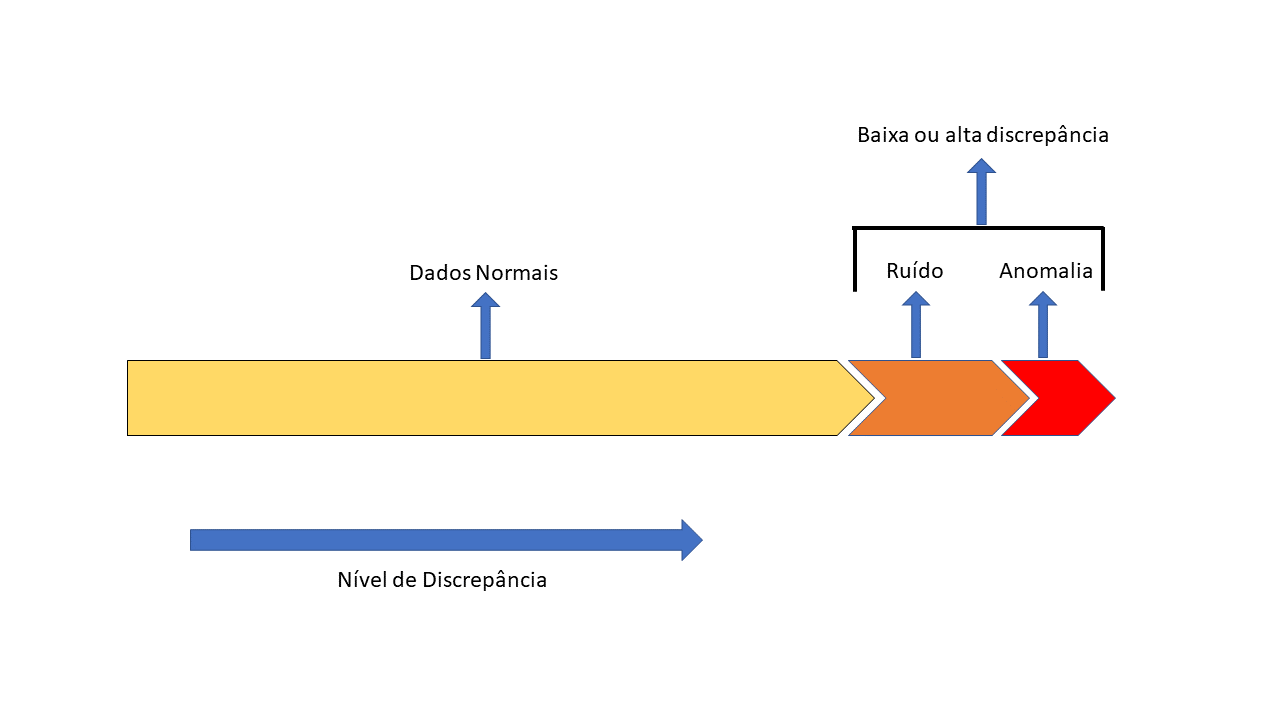
\includegraphics[width=\linewidth]{./figures/FundamentacaoTeorica/ExemploDeDiscrepancia.png}
			\caption{Exemplo de escala de discrepância (Adaptado de Aggarwal) }
			\label{fig:Aggarwal}
		\end{figure}
		

		%Como lidar com eles
		E se o dados discrepantes não forem tratados, eles podem gerar problemas como 
		redução da precisão do modelo de dados,
		aumentar a complexidade do modelo,
		dificultar e legibilidade dos dados também. \cite{Aggarwal2012} \cite{rathi_2019}
		E para tratá-los, as formas convencionais são 
		remoção de instâncias,
		filtro de dimensões,
		combinar essas formas convencionais com algoritmos de validação - como o k-fold - ou
		detecção de anomalias - como baseado em clusterização, SMV ou densidade.
	
		\subsection{Dados Ruidosos e Anômalos}
			%O que são dados ruidosos
			Dados ruidosos são dados indesejaveis, dimensões ou instâncias que não estão relacionadas com o fenômeno estudado. \cite{rathi_2019}
			Em geral, dados ruidosos fazem com que algoritmos de aprendizado de máquina encontrem padrões incoerentes. \cite{rathi_2019}
			Dados ruidosos e dados anômalos diferenciam-se, basicamente, na sua facilidade de percepção em uma visualização e no seu grau de impacto ao inferir sobre os dados.
			Na figura \ref{fig:ruidoAnomalo}, o item A é um exemplo de dado ruidoso, pois desvia-se levemente do padrão dos dados - uma reta.
			Quanto ao Item B este descaracteriza significativamente o padrão dos dados - este é um exemplo de dado anômalo.
			\begin{figure}[h!]
				\centering
				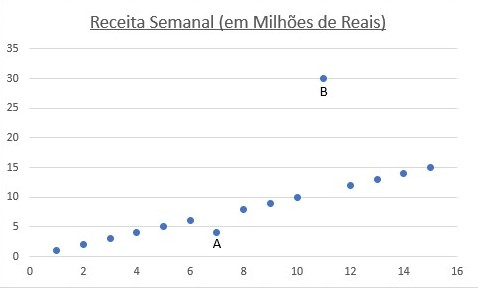
\includegraphics[width=\linewidth]{./figures/FundamentacaoTeorica/ExemploRuidoAnomalo.jpg}
				\caption{Exemplo de ruído e de anomalia.}
				\label{fig:ruidoAnomalo}
			\end{figure}
			\par
			
			%Quais os tipos
			Em dados tabulares, é possível classificar esses dados de 3 formas segundo \cite{rathi_2019} (ver figura \ref{fig:Rathi}),
			sendo estas abnormalidades,
			dimensões irrelevantes ou
			instâncias ruídas. 
			As abnormalidades são irregularidades tanto nas dimensões dos dados ou no evento estudado.
			As características irrevelentes são aquelas que não ajudam a explicar o fenômeno.
			E as instâncias ruídas são aquelas que desviam a forma dos outros dados. \cite{rathi_2019}
			\begin{figure}[h!]
				\centering
				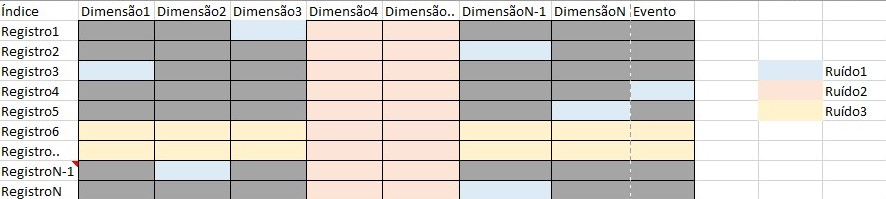
\includegraphics[width=\linewidth]{./figures/FundamentacaoTeorica/ExemploClassificacaoRuido.jpg}
				\caption{Exemplo das classificações de ruído (adaptado de Rathi)}
				\label{fig:Rathi}
			\end{figure}
			
\chapter{Trabalhos Relacionados}
	Nesse capítulo serão apresentados trabalhos acadêmicos e aplicações as quais possuem correlação com meu trabalho.
	Para isso, foram feitas análises sobre os trabalhos para identifcar semelhanças e diferenças pontuais.
	Essa análise foi feita com o fim de comparar os trabalhos e identificar contribuições, suprir necessidades e captar trabalhos futuros.

	\section{Trabalhos acadêmicos relacionados}
		Albuquerque et al. \cite{Albuquerque2011} descreveu um \emph{framework} capaz de gerar dados sintéticos multidimensionais.
		O sistema (ver figura \ref{fig:albuquerque}) recebe um \emph{input} que representa algumas propriedades do conjunto de dados como número de dimensões,
			uma distribuição de dados padrão,
			tipo de dado de cada dimensão entre outros.
		A partir disso, é criada uma função densidade de probabilidade, com o fim de gerar um cojunto de dados padrão.
		Essas funções podem ser ajustadas e modeladas através de objetos.
		Também, essas funções podem ser de 1, 2 ou 3 dimensões.
		Adicionalmente, pode-se haver ruídos, para simular as irregularidades encontradas em conjunto de dados reais.
		\par
		O framework apresentado também possui uma interface gráfica para auxiliar o usuário a configurar o conjunto de dados, bem como gerá-lo. Contudo, não foi encontrado uma interface para pré-visualização dos futuros dados gerados. Quanto aos tipos de dados, estes são restritos aos numéricos, quer sejam inteiros ou de ponto flutuante.    
		\begin{figure}[h!]
			\centering
			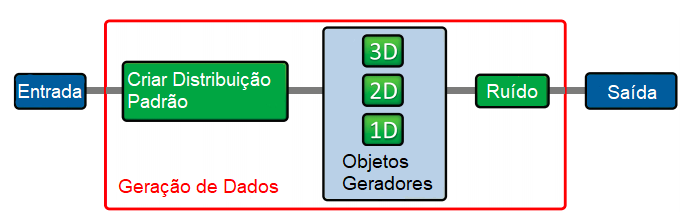
\includegraphics[width=\linewidth]{./figures/TrabalhosRelacionados/Albuquerque10.png}
			\caption{Visão Geral de geração de dados.}
			\label{fig:albuquerque}
		\end{figure}

		Wang et al. \cite{BingWang2013} apresentou uma aplicação cujo principal diferencial é a capacidade de modelar, através de desenho, o comportamento das dimensões do conjunto de dados sintéticos. A priori, o usuário pode iniciar o processo de geração através do zero, de um conjunto de dados já existente, ou um conjunto de dados aleatório. A partir disso, o usuário visualiza os dados no gráfico - que pode ser as coordenadas paralelas ou o \emph{scatterplot} - e pode modificá-lo através de cliques e arrastos. Por conseguinte, os dados podem ser gerados e isto também serve como retroalimentação do sistema. Na figura \ref{fig:sketchpad} é possível visualizar a visão geral do funcionamento do SketchPad.
		\begin{figure}[h!]
			\centering
			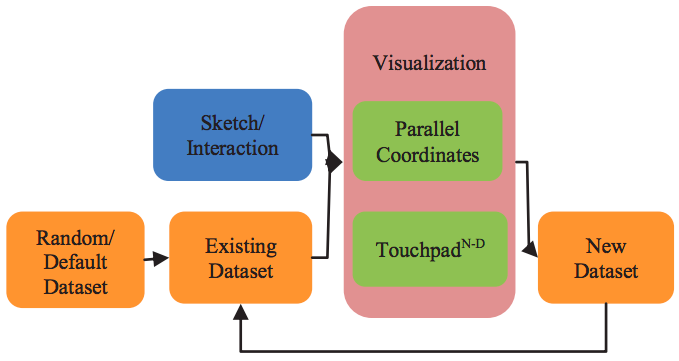
\includegraphics[width=\linewidth]{./figures/TrabalhosRelacionados/Wang11.png}
			\caption{Visão Geral de geração de dados do Sketchpad.}
			\label{fig:sketchpad}
		\end{figure}

		Liu \cite{Liu2016} criou um gerador de dados sintéticos a partir de avaliação de regras de aprendizagem. O sistema funciona criando regras de aprendizagem - usando algoritmos de árvore de decisão como o ID3 - baseado em dados de entrada contruindo correlações entre os dados. Na figura \ref{fig:liu} é possível visualizar uma árvore de decisão. Durante a leitura do conjunto de dados de entrada é feita a árvore de decisão e, concomitantemente, são geradas as regras de aprendizagem. Essas regras são utilizadas para gerar amostras de dados sintéticos.
		\begin{figure}[h!]
			\centering
			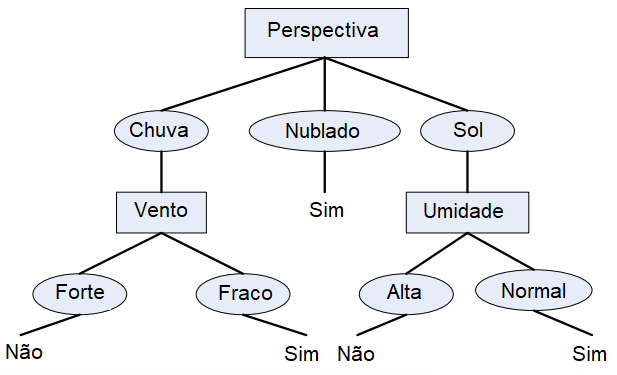
\includegraphics[width=\linewidth]{./figures/TrabalhosRelacionados/Liu13.png}
			\caption{Exemplo de árvore de decisão para jogar tennis criado a partir de regras encontradas em um conjunto de dados.}
			\label{fig:liu}
		\end{figure}

		Garcia e Millán \cite{Garcia2011} criaram um sistema par gerar dados sintéticos pensado para desenvolvedores que buscam testar de forma eficiente e exaustiva a sua aplicação. Esses dados pode ser configurados (ver figura \ref{fig:garcia}) de acordo com as preferências do usuário. As dimensões de dados seguem alguns padrões como a partir de fontes externas (Arquivos, Bibliotecas, Base de dados) Sequencial, Constante, Funcional, Intervalo ou Lista de valores. 
		\begin{figure}[h!]
			\centering
			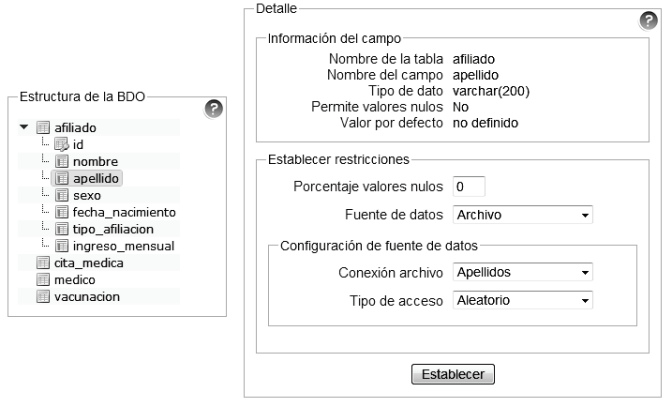
\includegraphics[width=\linewidth]{./figures/TrabalhosRelacionados/Garcia18.png}
			\caption{Exemplo da interface do usuário para configuração do gerador de dados.}
			\label{fig:garcia}
		\end{figure}

		Kofinas et al. \cite{Kofinas2018} criou uma metedologia para gerar dados sintéticos para simular consumo de água. A metodologia é avaliada através de algoritmos de validação - como a visualização dos resultados e fórmulas.
		\par
		Como pode ser visto na figura \ref{fig:kofinas}, a geração dos dados é feita a partir de 2 fases. A fase 1 serve, basicamente, para investigar a distribuição dos dados. Esta fase, primeiramente transforma dados números em séries temporais de 30 segundos. Em alguns casos, não há registro, para isso, é criada uma tabela de incidentes e posteriormente uma probabilidade de existência de registro para que seja encontrada as classes usadas para construção do histograma de Pearson \cite{dean2009descriptive}, por fim, são comparadas funções de distribuição com a atual com o fim de encontrar a que mais se aproxima.
		\par
		Para a fase 2 cuida da geração de dados sintéticos propriamente. Basicamente, o sistema utiliza a distribuição criada na fase um para gerar os dados para 24h, respeitando as características diferenciadas para dias de semana e finais de semana.
		\begin{figure}[h!]
			\centering
			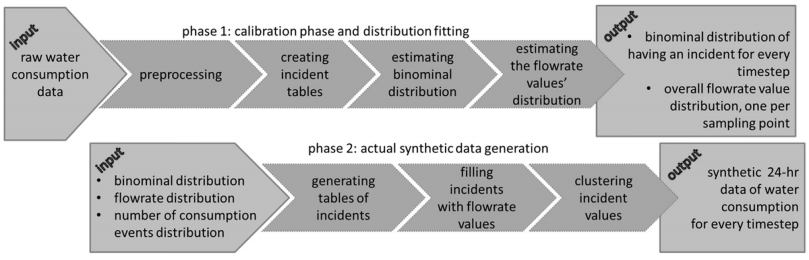
\includegraphics[width=\linewidth]{./figures/TrabalhosRelacionados/Kofinas21.png}
			\caption{Fluxo de passos para geração dos dados sintéticos.}
			\label{fig:kofinas}
		\end{figure}

		No trabalho feito por Sakshaug and Raghunathan \cite{Sakshaug2014} foi aplicado um procedimento de simulação não paramétrica para geração de dados sintéticos de variáveis contínuas com o foco em pequenas áreas geográfica. 
		Segundo a avaliação do autor os dados sintéticos tiveram validade moderadamente alta em seus testes, mas ressalta a limitação do método não paramétrico. 
		Em geral, os dados sintéticos se mostram promissores para geração de dados sintéticos para pequenas áreas geográficas, mas faltam testes mais aprofundados como dados de pesquisa em larga escala para substituir os dados reais por dados sintéticos em centros de dados de pesquisa.
		Na figura \ref{fig:SakshaugandRaghunathan} é possível observar a comparação dos resultados da média da simulação paramétrica e da não paramétrica para cada atributo.
		Na simulação não paramétrica as médias dos dados sintéticos e reais ficam bem próximas, com exceção da idade (\emph{age}), apresentando um bom resultado para a troca de dados reais para dados sintéticos.
		\begin{figure}[h!]
			\centering
			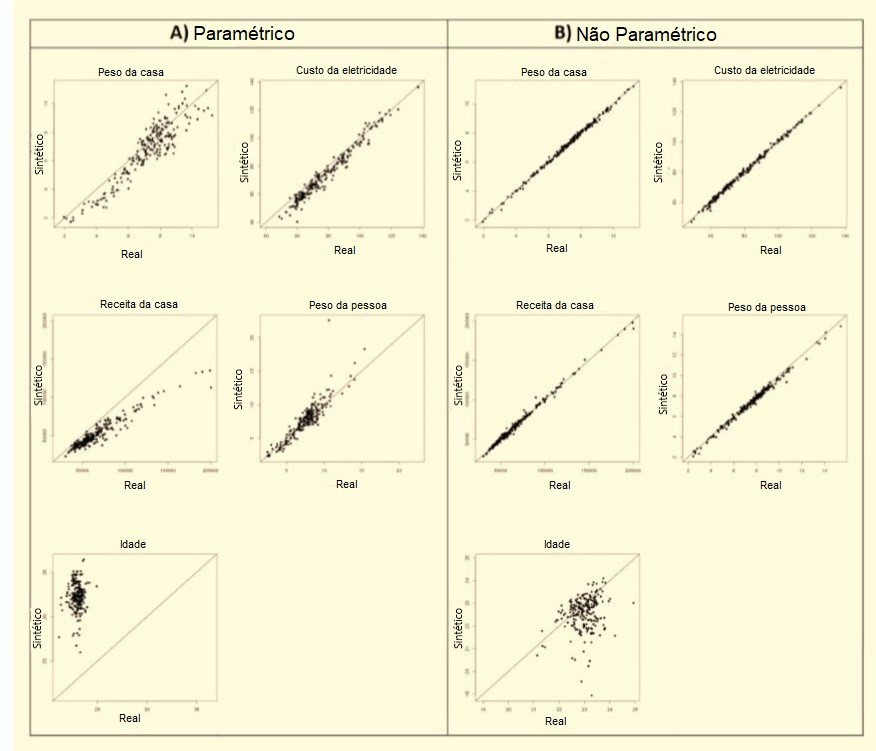
\includegraphics[width=\linewidth]{./figures/TrabalhosRelacionados/SakshaugandRaghunathan.jpg}
			\caption{Comparação da média dos dados reais e sintéticos na simulação paramétrica e não paramétrica.}
			\label{fig:SakshaugandRaghunathan}
		\end{figure}

		Similarmente ao Blocks Data Generator, o projeto Threat Streaming Generator (TSG) \cite{Whiting2008} visa criar um gerador de dados sintéticos realistas com foco em dados para testes.
		É mostrado o fluxograma dos processos do TSG na figura \ref{fig:whitingetal}.
		Primeiramente são definidos qual o tipo de conjunto de dados vai ser gerado.
		Em seguida são dadas 3 possilidades ao usuário de inserir o ambiente e a ameaça: manualmente, através da ferramenta TSG e outras fontes.
		Por fim, esses dados são analisados por especialistas os quais são responsáveis pela qualidade do conjunto de dados gerado.
		\begin{figure}[h!]
			\centering
			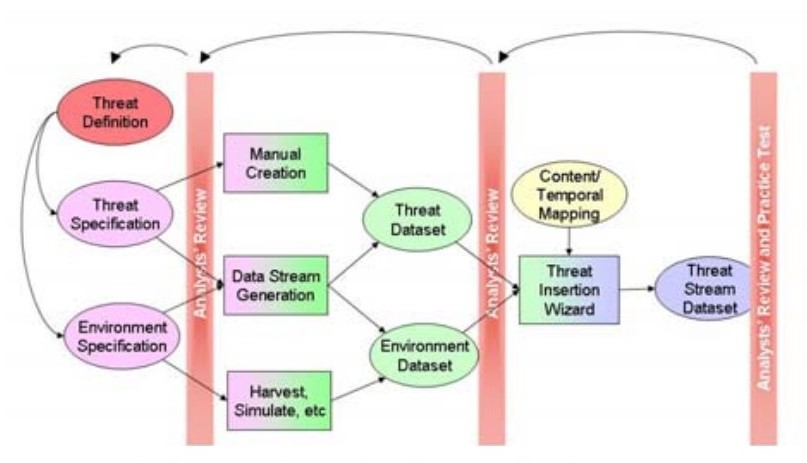
\includegraphics[width=\linewidth]{./figures/TrabalhosRelacionados/whitingetal.jpg}
			\caption{Fluxo de passos para geração dos dados sintéticos.}
			\label{fig:whitingetal}
		\end{figure}

		Com o foco em CARS (Context-Aware Recommender Systems - Sistemas de Recomendação sensíveis ao contexto), o DataGenCARS \cite{delCarmenRodrguezHernndez2017} é uam ferramenta para gerar dados sintéticos de forma flexível e prática.
		Permitindo que o usuário possa inserir os tipos perfis do usuário, tipos de contexto e itens, misturar dados sintéticos e dados reais com o fim de aumentar o realismos dos dados gerados.
		Na imagem \ref{fig:DataGenCARS} mostra-se, de forma geral, o funcionamento do DataGenCARS.
		De início a ferramenta mostra que é possível, opcionalmente, expandir outros conjuntos de dados bem como analisá-los estatisticamente.
		De qualquer modo, deve ser definido os esquemas de contexto usuários, itens e configuração da geração para que se tenha o conjunto de dados.
		\begin{figure}[h!]
			\centering
			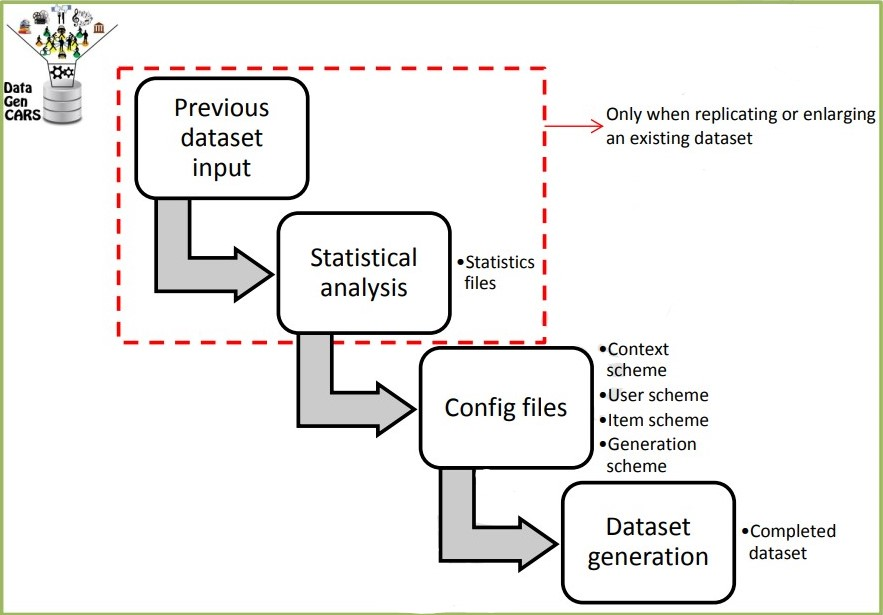
\includegraphics[width=\linewidth]{./figures/TrabalhosRelacionados/DataGenCARS.jpg}
			\caption{Fluxo de passos para geração dos dados sintéticos.}
			\label{fig:DataGenCARS}
		\end{figure}

		Pensando em oferecer confidencialidade dos dados governamentais, Larsen and Huckett \cite{Larsen2012} desenvolveram um gerador de dados sintéticos que alia regressão de quartis com imputação \emph{hot deck} e troca de classificação.
		A predição de regressão de quantis é feita para proteger dados sensíveis a partir de dados não sensíveis,
		 isto é, o conjunto de dados finais são compostos por dimensões reais - os não sensíveis - e sintéticos - para dimensões sensíveis.
		Em alguns casos os dados sintéticos são similares aos reais e para isso foi utilizado a imputação \emph{hot deck} junto com a troca de classificação, para garantir a aleatoriedade e confidencialidade dos dados.
		%Artigo sem imagem.

	\section{Aplicações relacionadas}

		DTM Data Generator \cite{DTMDataGenerator} é uma plataforma de geração de dados sintéticos que existe de 1998.
		Esta possui suporte para geração de dados em arquivos, em banco de dados, também para \emph{Big Data}.
		Possui suporte multiplataforma, através do modo \emph{multiplatform runtime}, contudo é limitado quando comparado à versão Windows, o qual suporta a versão para servidor também.
		É válido destacar que é um software essencialmente pago, isto é, existem versões gratuitas - demonstrações, para ser mais exato - mas limitadas.
		Além disso, há categorias de versões pagas, que vão desde limitações de geração (Standart - Professional) à vantagens mais técnicas (Professional - Entrerprise).
		\par
		O DTM Data Generator possui uma vasta coleção de funcionalidades, as quais liberadas de acordo com as versões pagas.
		Adotando a versão mais cara, a lista de \emph{features} é composta por geração de dados em JSON, XML, CSV ou geração por separador customizado.
		Também permite gerar dados por arquivo DSN (Database Source Name), gerar dados por linha de comando, e gerar um arquivo SQL para não seja necessário conexão com banco de dados.
		\par
		É possível gerar cerca de 9.2 sextilhões de registros por \emph{rule}, modos de atualizar dados existentes (adicionar, substituir e \emph{Data Scrambling}), e suporte para bibliotecas de dados realistas.
		A plataforma disponibiliza entrada de dados através de SQL, XML, JSON, pela WEB através de HTTP ou FTP, XLSM, arquivos de texto e scripts em Python.
		Também é possível visualizar e testar os dados gerados, bem como gerá-los nos principais arquivos de texto (TSV, CSV, "DSV", JSON, XML) e banco de dados. (MS SQL Server, Oracle, DB2, MySQL, PostgreSQL, Informix, Sybase, SQLite e Firebird) 
		\par
		Há uma suíte de produtos relacionados fornecidos pela DTM soft. 
		Além do gerador de dados, 
			há o gerador de dados XML para teste de aplicação (DTM Test XML Generator);
			um gerador de planilhas Excel (DTM Data Generator for Excel)
			testador exaustivo - teste de estresse - de banco de dados (DTM DB Stress);
			Bem como editor, visualizador (DTM Data Editor), comparador e sincronizador de banco de dados (DTM Data Comparer) entre outros. 
		\begin{figure}[h!]
			\centering
			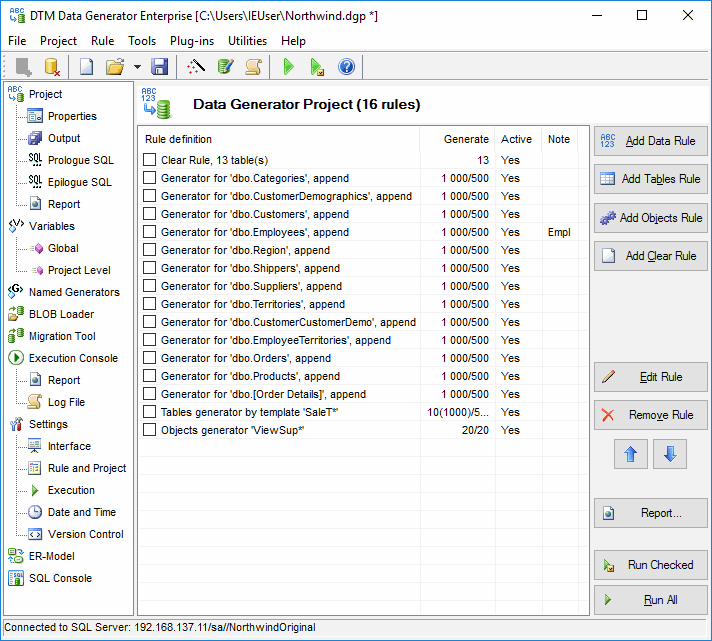
\includegraphics[width=\linewidth]{./figures/TrabalhosRelacionados/DTMDataGenerator.png}
			\caption{Usando o DTM Data Generator. Fonte: DTM Data Generator}
			\label{fig:DTMDG}
		\end{figure}

		O SQL Data Generator \cite{RedgateSQLDataGenerator} é um software que compõe uma suíte de ferramentas (chamada de SQL Toolbelt) da Red Gate.
		O software é exclusivo para o ecossistema Windows, com suporte do Windows 7 ao 10, à versão para servidores do Windows, ao SQL Server (2008 ao 2017), .NET e Oracle.
		Este produto é distribuido através de licenças pagas e vitalícias, com atualizações gratuitas e, no mínimo 1 ano de suporte gratuito.
		Vale ressaltar que é possível testar o produto por 14 dias gratuitamente.
		\par
		O SQL Toolbelt tem funcionalidades bem delimitadas e a função do Data Generator é popular um banco de dados. 
		A população acontece ao escolher, primeiramente, uma tabela do banco.
		A partir disso, escolhe-se um gerador para cada coluna da tabela.
		Um gerador tem classificação fortemente baseada na realidade, isto é, possui geradores como palavras relacionadas à compras, pagamentos, pessoas (primeiro e último nome), dado geográficos e afins.
		Contudo, também disponibiliza a geração a partir de expressões regulares \emph{Regex generator} e scripts de python.
		Por se tratar de banco de dados, também há checagem e tratamento de \emph{constraints}, \emph{Foreign keys} e \emph{Dependencies}.
		O SQL Data Generator também permite lidar com arquivos XML, quer seja para geração de valores XML, como utilizar como dados de entrada, além de mesclá-los com o \emph{Regex generator}.
		\par
		Quanto ao SQL Toolbelt oferecido pela Red Gate, ele conta com 2 modalidades, o completo com 14 programas e o \emph{essentials} com 10.
		Entre os mais relevantes, pode-se citar o \emph{SQL Data Compare}, \emph{SQL Data Generator}, \emph{SQL Test}, \emph{SQL Backup Pro} e \emph{SQL Scripts Manager}.
		\begin{figure}[h]
			\centering
			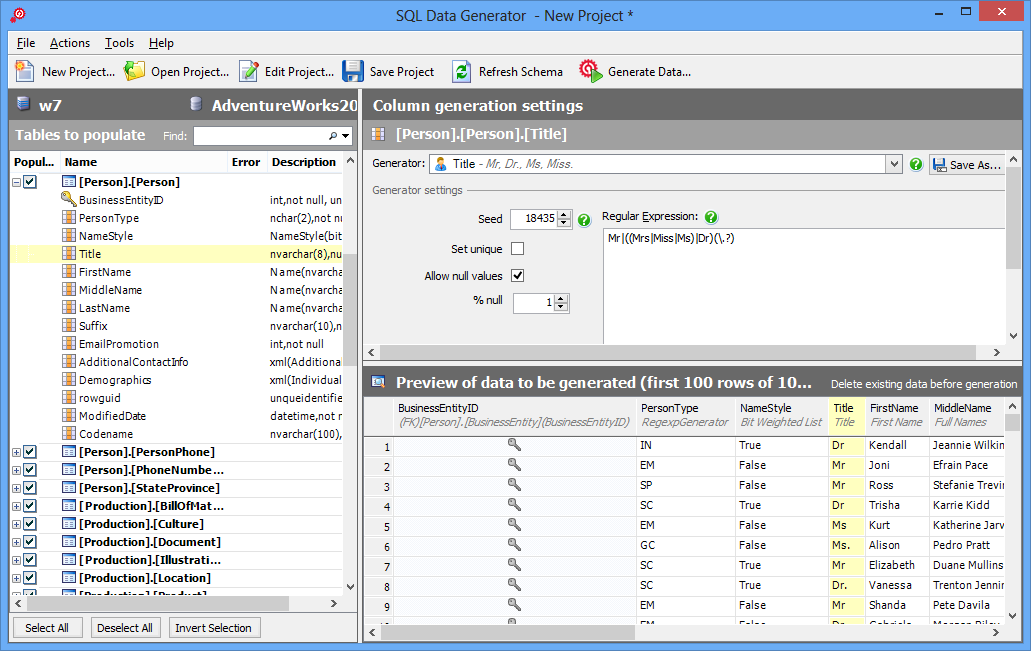
\includegraphics[width=\linewidth]{./figures/TrabalhosRelacionados/sql-data-generator.png}
			\caption{Usando o Redgate SQL Data Generator. Fonte: Red Gate SQL Data Generator.}
			\label{fig:RedgateSQLDG}
		\end{figure}

		Microsoft Visual Studio \cite{VSDataGenerator} é um pacote de programas da Microsoft para desenvolvimento de \emph{software}. 
		Este é composto por 4 versões (\emph{Express}, \emph{Professional}, \emph{Premium}, \emph{Ultimate}), e a opção de gerar dados para teste está disponível a partir da versão \emph{Premium}.
		O foco é permitir que verique o comportamento do banco de dados, sem relacioná-los com os dados da aplicação em produção.
		\par
		Para gerar os dados de teste, deve-se utilizar os geradores de dados (\emph{Data Generators}), que são correlacionados às tabelas do banco de dados.
			Os geradores podem ser dos mais primitivos (Binários, Inteiros, Data, \emph{Float}), como de Imagem, Dinheiro, Expressão Regular, Categórico entre outros.
		Também é disponibilizado um Plano de Geração de Dados (\emph{Data Generation Plan}), feito em XML, que contém informações do banco de dados, o tipo de dados de cada gerador e a quantidade de dados para ser gerado. 
		Este plano serve basicamente para reutilização da lógica de teste.
		\begin{figure}[h]
			\centering
			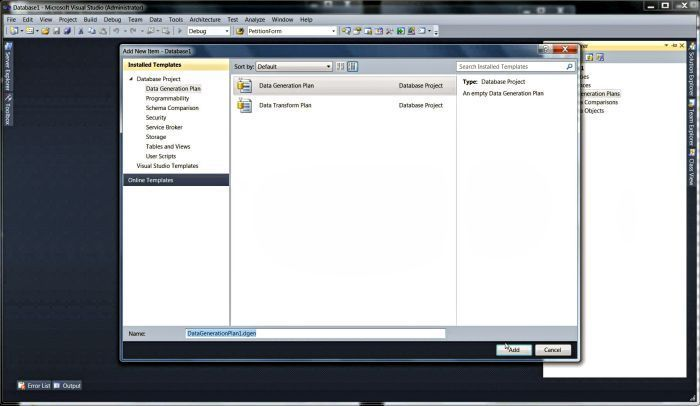
\includegraphics[width=\linewidth]{./figures/TrabalhosRelacionados/Visual-Studio.jpg}
			\caption{Usando o Microsoft Visual Studio. Fonte: anranik.}
			\label{fig:VSDG}
		\end{figure}

		Test Data Generator \cite{forgeDBDataGenerator} é uma ferramenta GUI (\emph{Graphical User Interface}) pela dbForge para gerar dados de teste para banco de dados SQL desde 1997.
		O software possui mais de 200 geradores predifinidos e configuráveis os quais permitem a geração de dados mais inteligentes, isto é, mais próximos da realidade, como nomes, localização, dados de saúde e afins.
		Quanto à compatibilidade, este é exclusivo do ecossistema Windows, com suporte à versão 7 ao 10, do Windows Server 2008 ao 2019 e ao SQL Server Azure, 2008 ao 2017.
		Além da GUI, também há o suporte para geração de dados a partir da linha de comando.
		O produto é distribuido sob licenças pagas e vitalícias, porém, com suporte ao cliente com tempo limitado e com 30 dias gratuitos para avaliação.
		\par
		Para usar o dbForge Test Data Generator, é preciso fazer uma conexão com banco de dados. 
		A partir disso, utiliza-se os \emph{Data Generators} para determinar o comportamento dos dados para determinada coluna da tabela selecionada no Banco de dados.
		Os Geradores de dados podem ser do tipo emph{Basics} e emph{Advanced}. 
		Do primeiro tipo, são formas mais próximas dos dados primitivos, como datas, texto \emph{lorem ipsum}, JSON, \emph{ReGex}.
		Já o avançado conta com número de cartão de crédito, aniversário, número de conta bancária internacional, IPv4, \emph{hash} de senhas.  
		A geração de dados resume-se à população de banco de dados, não há uma forma de exportar os dados em arquivos como CSV e JSON.
		\par
		Há um suíte exclusivo para SQL Server, contudo também para Oracle, MySQL, PostgreSQL entre outros.
		Neste suíte, há várias ferramentas que auxiliam na manutenção, mas não, necessariamente, a geração de dados, a exemplode um \emph{previewer}.
		Destes, pode-se citar um comparador de dados, criador de \emph{querys}, um monitor - para supervisão do banco de dados - e afins.
		\begin{figure}[h]
			\centering
			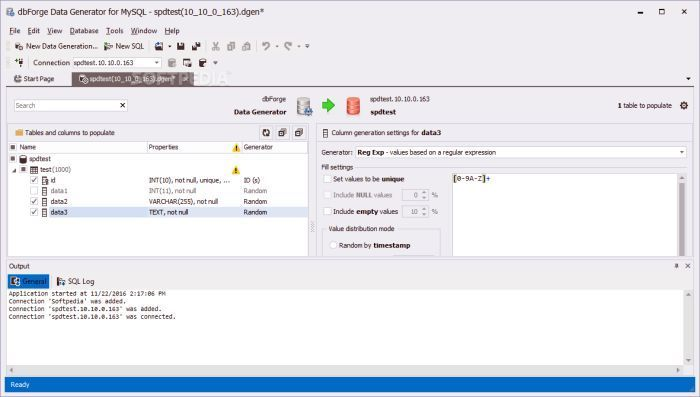
\includegraphics[width=\linewidth]{./figures/TrabalhosRelacionados/dbForge-Test-Data-Generator.jpg}
			\caption{Usando o dbForge Test Data Generator. Fonte: anranik.}
			\label{fig:dbForgeTDG}
		\end{figure}

		Mockaroo \cite{mockaroo} é um \emph{web site} e \emph{framework} para desenvolver dados de teste.
		Há um total de 143 geradores, sendo a maioria considerados geradores realistas.
		Por ser um site, é possível acessá-lo por qualquer sistema operacional, dependendo apenas de conexão com a internet.
		O produto possui versões gratuita e pagas. - \emph{Free}, \emph{Silver}, \emph{Gold}, \emph{Enterprise} as quais variam no \emph{host}, o qual pode ser do Mockaroo ou privado, máximo de registros por download, velocidade de download e preço.
		\par
		Na tela inicial, é possível escolher o nome da coluna, o tipo de gerador, algumas opções - valores em branco e funções a partir dos dados.
		Ainda nesta tela, encontra-se o botão para \emph{download} dos dados, pré-visualização dos mesmo (mas sem gráficos), algumas configurações como quantidade de linhas, formato dos dados para \emph{download}, botão para clone ou deleção de banco de dados, e importação de dados csv/Excel ou SQL.
		\par
		Outro serviço interessante do Mockaroo é Mockaroo APIs \cite{mockarooAPI}.
		Este consiste em baixar dados programaticamente através de requisições REST (\emph{Representational State Transfer}).
		As requisições podem ser feitas de 2 formas, a \emph{Generate API} - gera os dados através de um banco de dados salvo e os envia pelo corpo de uma requisição - 
		e \emph{Mock APIs} que basicamente, simula um \emph{back-end} como tratamento de parâmetros e simulação de erros. 
		É pensado para desenvolvimento ágil de aplicações \emph{front-end}, isto é, sem perder muito tempo com o \emph{back-end} a priori.
		\begin{figure}[h]
			\centering
			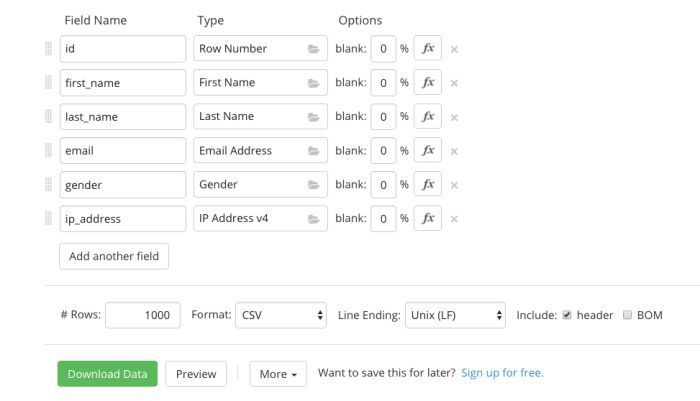
\includegraphics[width=\linewidth]{./figures/TrabalhosRelacionados/mockaroo.jpg}
			\caption{Usando o Mockaroo. Fonte: anranik.}
			\label{fig:mockaroo}
		\end{figure}
		% \subsubsection{ApexSQL Generate}
		% \subsubsection{Datanamic Data Generator MultiDB}
		% \subsubsection{Upscene Advanced Data Generator}
		% \subsubsection{EMS Data Generator}
		% \subsubsection{GEDIS Studio}

		
	% ---
\chapter{Arquitetura do projeto}\label{cap_trabalho_academico}
% ---

%-- TODO: 
	%Inserir os Casos de Uso
	%Inserir as ferramentas utilizadas
	O software chamado de Blocks Data Generator é \emph{Open Source} e está hospedado no GitHub em \url{http://github.com/gustavoresque/DataGenerator}.
	Em termos de organização do projeto, foi adotado um modelo incremental de desenvolvimento, com reuniões diárias para discussão de problemas e melhorias, e utilização da ferramenta Trello (\url{https://trello.com}) para organização das informações, problemas e melhorias.
	\par
	Em termos de desenvolvimento, foi utilizada a linguagem Javascript com foco para \emph{Desktop}, através do \emph{Framework} Electron (\url{https://electronjs.org/}).
	Adotando o padrão de projeto MVC (\emph{Model, View, Controller}), também foi adicionado o \emph{jQuery} para agilizar a codificação do projeto.
	Do Javascript também foi utilizado o Node.js (\url{https://nodejs.org/en/}) para acessar recursos do sistema operacional, para o desenvolvimento do \emph{Web Service} e também para dar suporte ao Electron.
	E quanto à versão do Javascript foram utilizados os novos recursos do Ecmascript 6 (2015) como o desenvolvimento assíncrono com as \emph{Promises} e \emph{arrow functions}.
	
	\section{Casos de uso do sistema}
		\begin{figure}[h!]
			\centering
			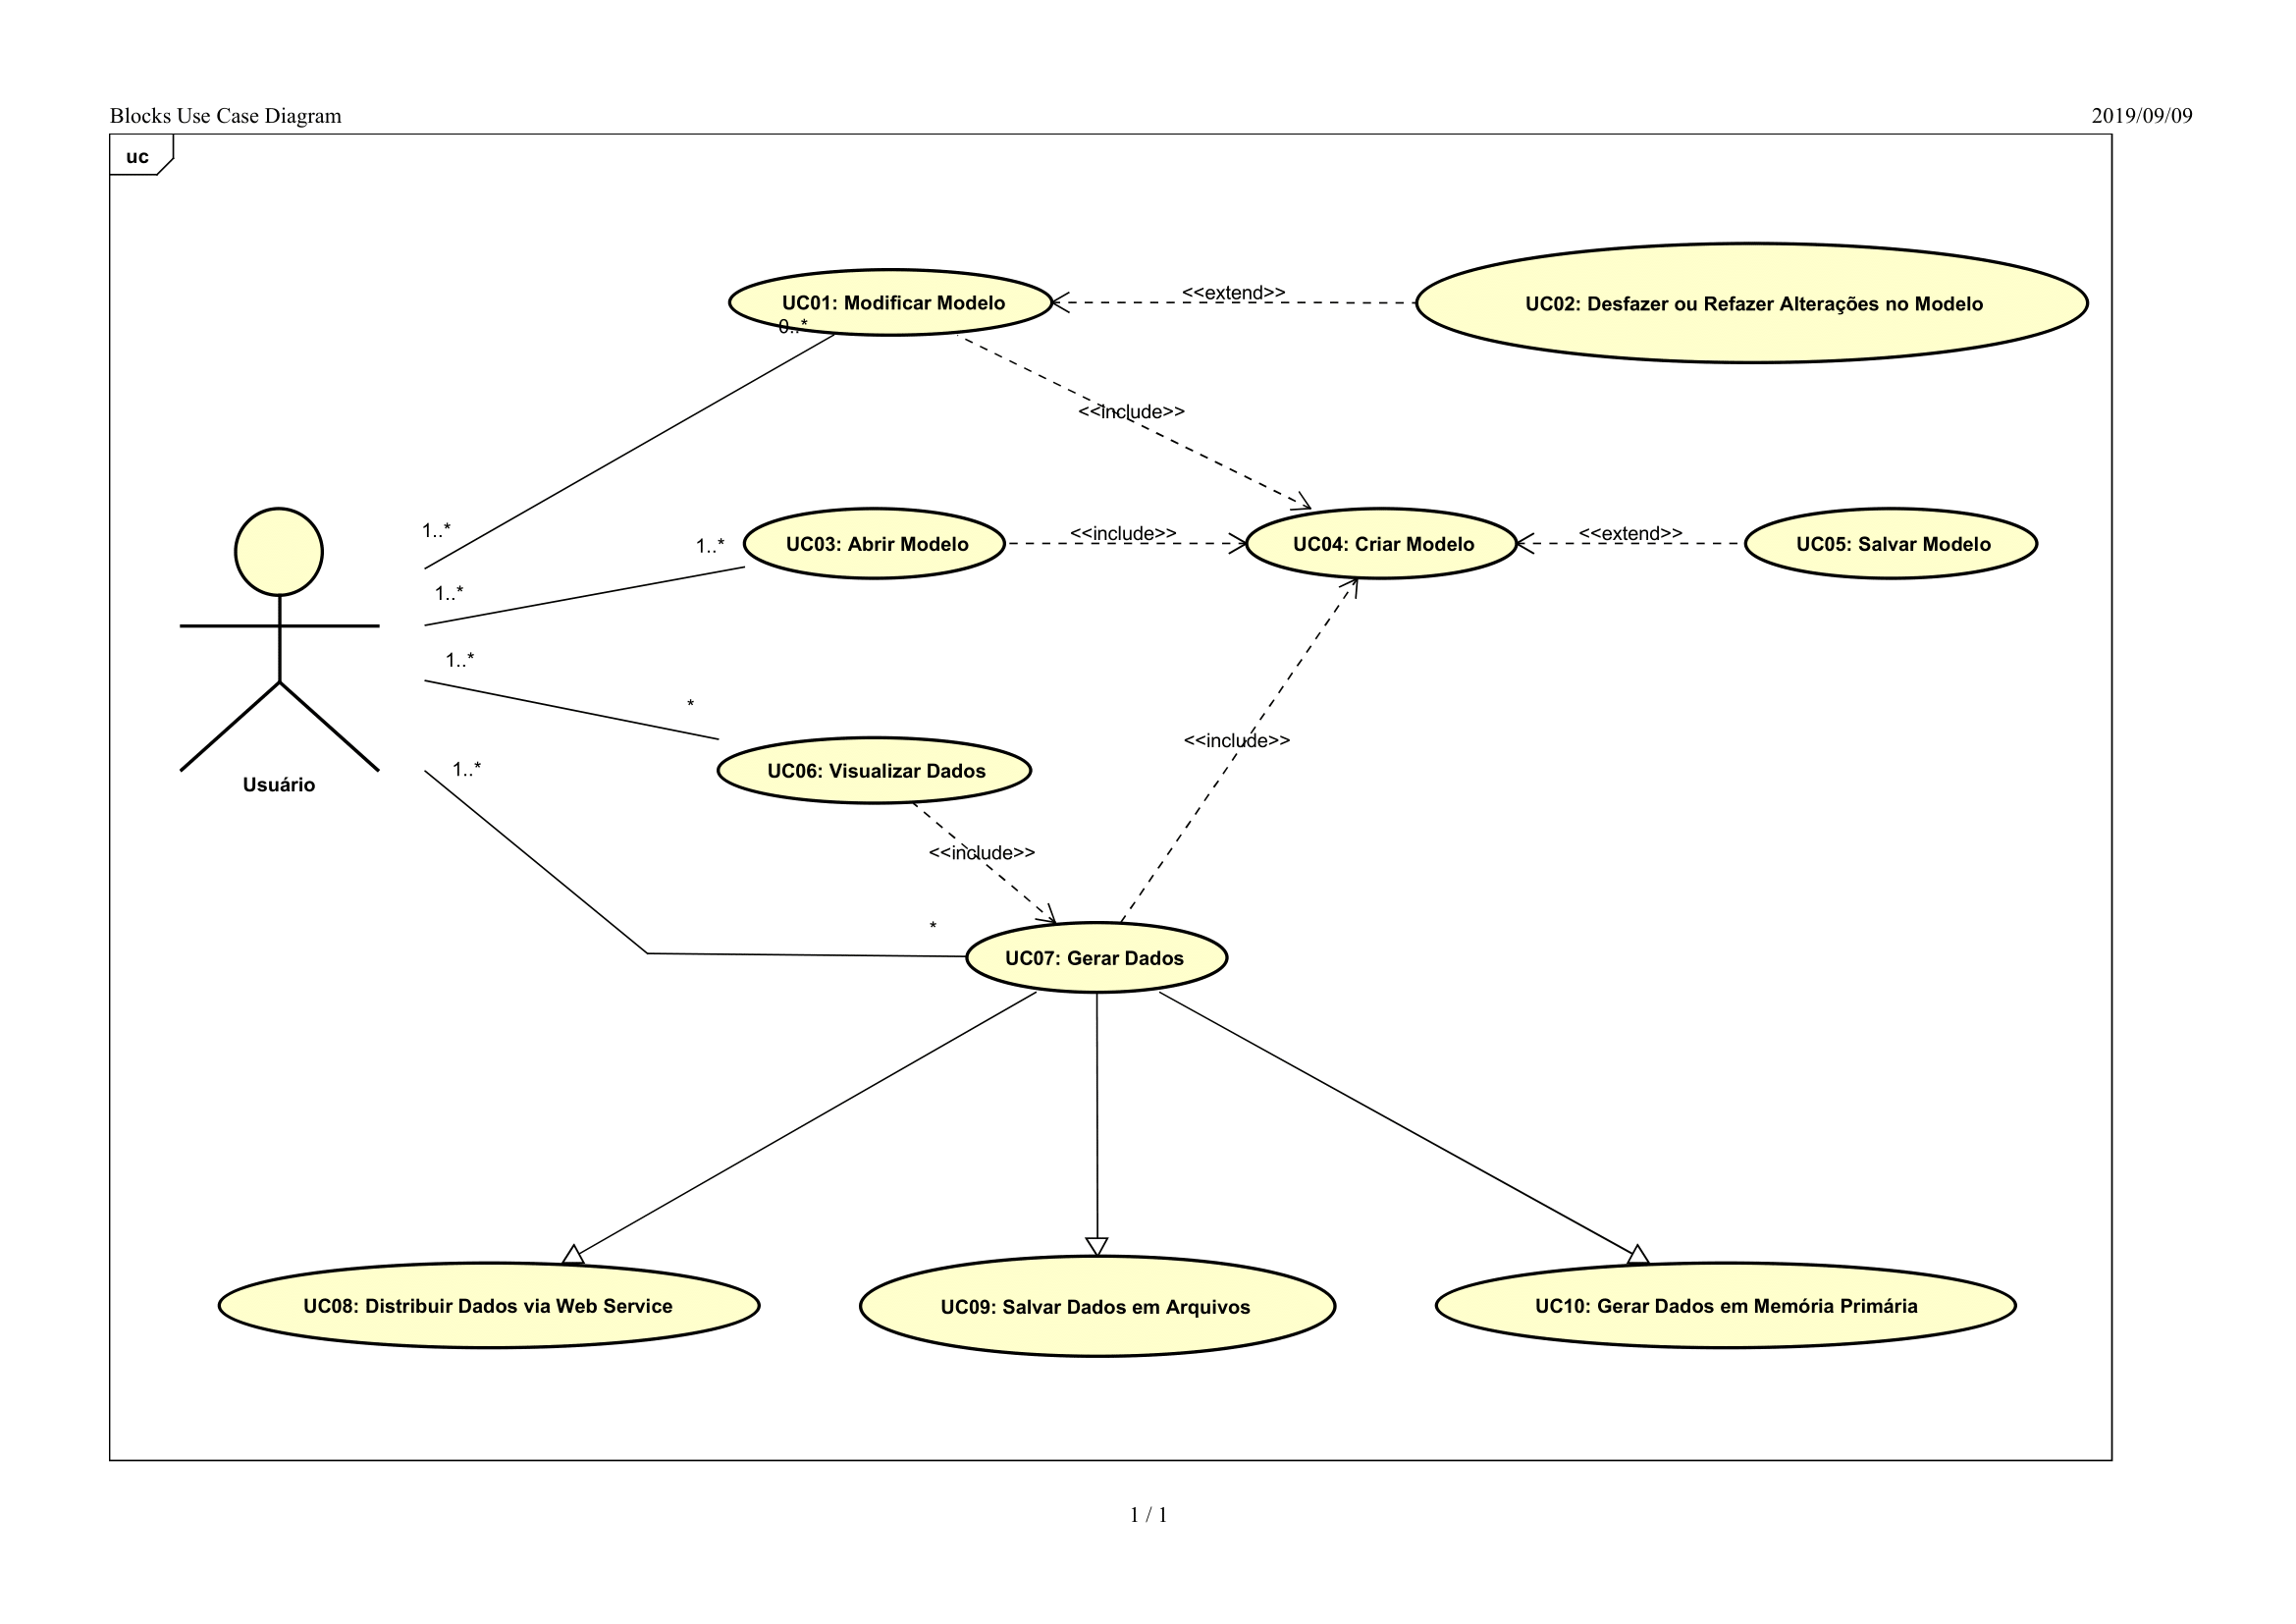
\includegraphics[width=\linewidth]{./figures/prototipo/diagramaUC.png}
			\caption{Diagrama de Caso de uso do Blocks Data Generator. Fonte: o autor.}
			\label{fig:diagramaUC}
		\end{figure}
		"O objetivo de um diagrama de casos de uso na UML é demonstrar as diferentes maneiras pelas quais um usuário pode interagir com um sistema." \cite{UCdefinition}
		Por conta disso, é utilizado o Diagrama de Casos de Uso para demonstrar as principais funcionalidades do protótipo Blocks Data Generator.
		Na figura \ref{fig:diagramaUC} são encontrados um total de 10 casos de uso.
		No UC01 mostra que é possível modificar um modelo, isto é, adicionar ou remover dimensões, alterar geradores e afins; também há inclusão do UC04 e a possibilidade de desfazer ou refazer as alterações (UC02).
		O UC04 representa a criação do modelo. 
		Está é considerada a funcionalidade original, pois é incluída por vários e não inclui nenhuma funcionalidade.
		Outros que possuem relação com UC04 é o UC03 e UC07 como inclusão e UC05 como extensão.
		\par
		UC03 é uma funcionalidade para reaproveitamento do modelo, também está atrelado à validação de teste por outros pesquisadores.
		UC07 é o carro chefe do Blocks Data Generator, o qual refere-se à geração de dados, progredindo para o \emph{Big Data} ou não.
		Esta geração pode ser feita, especificamente, de 3 formas: gerando dados em Memória, para ser utilizado dentro do sistema (UC10);
			salvar em arquivos - TSV, CSV e JSON - (UC09);
			e distribuir os dados através de requisições HTTP (UC08).
		\par
		Incluindo a UC07, mais especificamente a UC10, a UC06 permite que o usuário visualize os dados. 
		Assim, a visualização - a qual pode ser rápida (através do \emph{preview}) ou detalhada (com o VisTechLib) - tendo um panorama do comportamento dos dados. 
		Com isso, pode-se validar os dados, ter insights para aprimorar o modelo e afins.

% ---
\chapter{Protótipo}
% ---
	Este capítulo é dedicado em explicar mais sobre o prótótipo, seu fluxo de funcionamento, funcionalidades, mais detalhes sobre a interface do usuário entre outros.
	De modo geral, o protótipo é chamado de Blocks Data Generator e visa ser um gerador de dados sintéticos baseado em modelos de dados.
	Assim, o usuário pode manipular um ou mais modelos e cada modelo pode conter N dimensões, que por sua vez podem conter M geradores de dados encadeados.
	\par
	Os geradores de dados podem gerar dados numéricos, categóricos, temporais etc (haverá uma seção específica para geradores) e o resultado de um gerador pode servir de entrada para outro gerador através de operadores.
	Os operadores podem ou não aplicar uma operação matemática (soma, subtração, divisão, multiplicação) ao resultado do gerador anterior - a leitura de anterior e posterior é da esquerda para a direita, respectivamente.
	Junto com os operadores, também há outras propriedades que variam de acordo com o gerador (ver seção 4.1).
	\par
	Ainda na modelagem das dimensões, é possível modificar seu nome, verificar o tipo do dado gerado pelo gerador, o ID e se está disponível para geração e visualização.
	Essa disponibilidade (chamado de \emph{display}) foi feita para o caso de haver um modelo em que nem todas as dimensões sejam necessárias em determinado momento, mas também não queira perdê-las.
	Adicionalmente, é possível copiar e colar dimensões através de atalhos no teclado, bem como adicionar ou excluir dimensões, esta por só meio de um botão.
	\par
	Também é disponibilizado um pré-visualizador de dados com apenas um gráfico - o coordenadas paralelas -, cujo volume de dados é independente do volume de dados para ser gerado, colorido e interativo.
	Além do \emph{preview}, há uma integralização com um visualizador de dados mais elaborado e com mais opções de visualização.
	\par
	Outrossim, há um botão específico para gerar os dados em arquivos JSON, CSV, TSV ou por de requisições HTTP do tipo GET (\emph{Web Service}).
	Vale ressaltar que quantidade de dados gerados, pré-visualizados, formato dos dados gerados e se contém a legenda dos dados no arquivo final é configurável em ambiente especializado, assim como para o \emph{Web Service}.
	\begin{figure}[h]
		\centering
		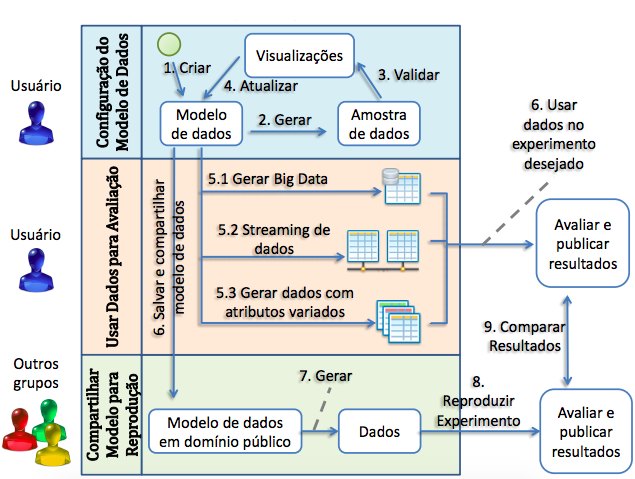
\includegraphics[width=\linewidth]{./figures/prototipo/fluxogramaUtilizacaoBlocks.png}
		\caption{Fluxograma de utilização do Blocks Data Generator Fonte: Yvan Brito, 2019.}
		\label{fig:fluxograma}
	\end{figure}
	\par
	Na figura \ref{fig:fluxograma} é possível visualizar como foi pensada a utilização da aplicação.
	Na primeira raia, encontra-se como usuário pode configurar o modelo.
	Basicamente, o usuário define as dimensões e os seus geradores e o comportamento dos dados pode ser validado pelo \emph{preview}, se precisar o modelo pode ser atualizado a qualquer momento.
	\par
	A segunda raia demonstra os caminhos para geração de dados.
	É possível a geração de dados por \emph{Big Data}, isto é, um grande conjunto de dados multidimensionais, apenas por meio de arquivos.
	Também a geração de dados por \emph{Streaming}, o qual dar mais controle ao usuário sobre o processo de geração, e também é disponibilizado o \emph{Web Service}.
	E o caminho 5.3 demonstra uma for iterativa de geração de arquivos de dados, com mudanças programadas de atributos.
	Esses dados podem ser usados em experimentos, testes e afins, cujos resultados podem ser publicados.
	\par
	A terceira raia funciona como um agrupamento das duas primeiras, mas externa.
	Isso para demonstrar que os processos anteriores podem ser replicados a partir do mesmo modelo de dados e o resultado pode ser comparado, facilitando Método Científico de pesquisadores sérios.
	
	\section{Tipos de Geradores de Dados}
		% TODO: colocar as fórmulas na seção de fórmulas (perguntar para o professor antes)
		\subsection{Sequencial}
			Os geradores da categoria Sequencial geram valores encadeados dado um padrão.
			É possível gerar o próprio padrão a partir do gerador \emph{Custom Sequence}, o qual você determina um valor Inicial (\emph{Begin}), o valor Intervalar (\emph{Step}), isto é, o qual vai ser incrementado ou decrementado dado uma Sentencia (\emph{sentence}) customizada.
			\par
			Contudo, já são predefinidos alguns geradores como 
				o \emph{constant}, o qual define um valor único de geração;
				o \emph{counter}, funciona como um contador, onde-se é definido o valor Inicial e o Intervalar;
				o \emph{Fixed Time Generator} gera um intevalo de tempo, onde-se define o valor inicial (\emph{init}), Intervalar e a máscara (\emph{mask}), isto é, como o tempo deve ser formatado;
				o \emph{Sinusoidal Sequence} gera de acordo com a função senoidal, que, além do valor Inicial e Intervalar, há o 'a' de Amplitude, 'b' de frequência ângular e 'c' para representar a fase da onda.

		\subsection{Aleatório}
			A categoria aleatória de dados são as que contem mais geradores, pois são mais fáceis de se dissociar da realidade, pelo caráter aleatório, mas também de reaproximar, pelo caráter probabilístico.
			\par
			Esta categoria conta com geradores uniformes, isto é, a distribuição dos dados é equalizada;
				Também há um gerador de dados de tempo, parecido com o \emph{Fixed Time Generator} com a diferença que o comportamento é definido pela fórmula de Poisson e que há mais duas configurações: unidade de tempo - a qual pode ser desde milissegundos a anos - e o lambda, advindo da fórmula.
				Há uma distribuição de poisson também, apenas com o lambda;
				É disponibilizado geradores de fórmulas clássicas com a normal (Gaussiana), Bernoulli, e Cauchy com seus devidos parâmetros.
			\par
			Além de números, também é possível gerar dados categóricos (\emph{Categorical}), dadas as palavras inicialmente.
				Similarmente há o \emph{Weighted Categorical} que possui valores de probabilidade para cada palavra, e 
				já o \emph{Categorical Quantity}, em vez de probabilidade, define quantas vezes cada palavra deve aparecer.
		\subsection{Funcional}
			A categoria funcional \emph{Function} serve para gerar dados de acordo com outra dimensão chamado de \emph{input}, isto é, facilita a correlação entre dimensões.
			Para dados numéricos, disponibiliza-se as 
				função de primeiro \emph{Linear Function} e 
				segundo \emph{Quadratic Function} grau, 
				exponencial \emph{Exponential Function}, 
				logarítmica \emph{Logarithm Function} e
				a \emph{Piecewise Function}, cuja função é definida por subfunções, e no caso, é possível definir o gerador desejado até um determinado valor chamado de \emph{Intervals} e depois pode-se escolher outro gerador.
			\par
			Para dados categóricos, há a função categórica \emph{Categorical Function} e 
			a \emph{TimeLaps Function} a qual funciona de forma semelhante ao gerador \emph{Piecewise Function}, só que utiliza uma quantidade de tempo como limiar, chamado de \emph{Laps} e também somente geradores de tempo como \emph{input}.
		\subsection{Acessórios}
			Os geradores da categoria Acessórios (\emph{Acessory}) foram pensados especialmente para serem concatenados com outros geradores, com o fim auxiliá-los.
			Entre os geradores acessórios, pode-se citar o \emph{Missing Value}, o qual retira alguns dados do conjunto;
			%TODO: Adicionar novos tipos de missing value.
				o \emph{Noise Generator} que adiciona dados fora do padrão, conhecido como ruído, com uma determinada probabilidade e intensidade*
				o \emph{Constant Noise Generator} também adiciona ruídos, mas só que é um valor específico com determinada probabilidade de ser adicionado;
				o \emph{Ranger Filter} permite ficar no conjunto de dados apenas os valores que estão entre os valores de início \emph{Begin} e fim \emph{End};
				o \emph{Linear Scale} permite que os determinados (selecionados através do \emph{MinIn} e \emph{MaxIn}) dados sejam escalados através do \emph{minOut} e \emph{MaxOut}.
			\par
			O \emph{No Repeat} retira dados repetidos do conjunto;
				o \emph{MinMax} define quais valores serão os maiores e menores de acordo com os parâmetros dados;
				o \emph{Low-Pass Filter} faz jus ao nome e filtra pela "Amplitude" do dado. Na prática, o valor sucesso é uma media ponderada (valor recebido pelo parâmetro \emph{Smooth}) do valor anterior com o valor gerado;
				o \emph{Get Extra Value} pega os retornos extras dos geradores que retornam mais que um valor.
		\subsection{Geométrico}
			A categoria de geradores Geométricos (\emph{Geometric}) permitem que o usuário desenhem o comportamento dos dados, através da ferramenta de desenho no sistema.
			Para isso são disponibilizados dois geradores.
			O primeiro gerados bidimensionais a partir da linha desenhada pelo usuário (\emph{Path2D Stroke}).
			Quanto ao segundo, este gerado os dados a partir do preenchimento da linha desenhada (ver algoritmo \emph{Floodfill}) pelo usuário (\emph{Path2D Fill}).
		\subsection{Baseado em dados reais}
			Para esta categoria, existe apenas um gerador, chamado como \emph{Real Data Wrapper}.
			Basicamente, ele é criado automaticamente quando o usuário importa um conjunto de dados reais através de um CSV, por exemplo.
			Este gerador recebe tantos valores categóricos como numéricos e essa informação pode ser decidida automaticamente pelo gerador ou ser forçada pelo usuário.
			É possível gerar uma quande superior de dados do que do conjunto de dados real, para isso é feito um tratamento para dados faltantes.
			Esse tratamento é feito através de funções de geração, chamadas de \emph{GenType}.
			\par
			Essas funções pode ser do tipo \emph{Standart}, que é pegar os dados do início ao fim de forma cíclica até chegar ao número desejado de registros.
			Também pode ser do tipo \emph{Reverse} que ao invés do \emph{Standart}, pega os dados do final ao início.
			É disponibilizado o modo aleatório (\emph{Random}), e algumas variações.
			\par
			A primeira variação é o \emph{QuartileRandom}, que divide o conjunto de dados em 3 marcos e a probabilidade de se pegar um dado daquele quartil é proporcional ao tamanho do marco.
			A leitura dos Marcos pode ser visualizada na figura \ref{fig:leituraMarco}. Então, se o valor do espaço entre 0 e quartil 1 for 100, todos os dados gerados serão do primeiro 1/4 do conjunto de dados.
			A segunda variação é o \emph{AverageRandom} que utiliza o valor da média e da variancia - [Média - Variancia, Média + Variancia] de um conjunto de dados númerico ou utiliza os N valores categóricos mais frequentes com distribuição uniforme.
			\begin{figure}[h]
				\centering
				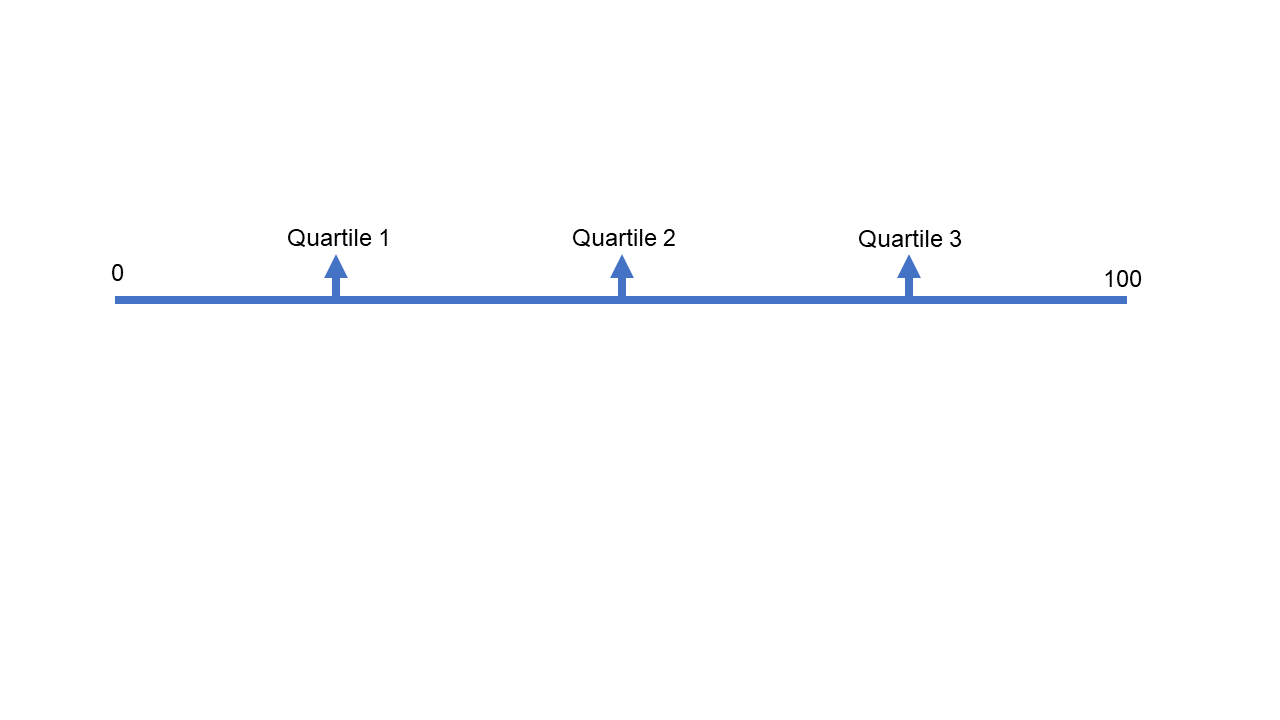
\includegraphics[width=\linewidth]{./figures/prototipo/quartil.png}
				\caption{Ilustrando a leitura dos marcos dos quartis. O tamanho do espaço entre os quartis ou entre 0 ou o 100 é o valor da probabilidade de um número ser desse espaço. Fonte: O Autor.}
				\label{fig:leituraMarco}
			\end{figure}
	\section{Modos de Geração de Dados}

		\subsection{Padrão e \emph{Streaming Data}}
			O protótipo, para uma quantidade limitada de registros e dimensões (5000 e 30 respectivamente) gera os dados agilmente, isto é, bloqueia a interface do usuário, para geração dos dados seja consistente com o modelo.
			O \emph{Streaming Data} foi pensando para o \emph{Big Data}. Então, quando foi passado o limiar da geração padrão dos dados, é criada uma cópia do modelo, para que o usuário seja livre para fazer alterações.
			E para fazer valer essa liberdade, o usuário tem o controle sobre o processo de geração por ver seu progresso e também poder cancelá-lo.
		\subsection{Web Service}
			Quanto ao \emph{Web Service}, este foi pensado para facilitar o teste de aplicação.
			Cada modelo é independente, isto é, podem ser habilitados somente os modelos desejados para distribuição.
			É além da configuração por dentro do \emph{software}, também é possível criar configurações temporárias para cada requisição, sem alterar as configurações o modelo.
			\par
			Os parâmetros disponíveis para configuração temporária pela URI são o nome do modelo, o formato dos dados e a quantidade de registro.
			É disponibilizado um aviso ao usuário quando um modelo está distribuindo dados via \emph{Web Service} na aba do modelo.
			Um exemplo de URI para fazer requisição HTTP do tipo GET (\url{http://localhost:8000/?modelid=MODEL_r6w2ffk3.mva&nsample=100&format=csv}), nos quais "modelid" é o \emph{ID} do modelo, "nsample" é a quantidade de registros desejado e "format" é o formato dos dados desejado.
	 
	\section{Modos para Visualização de Dados}

		
		\subsection{Footer Display}
		%Falar sobre o pequeno display no footer

		\subsection{Preview}
			O pré-visualizador de dados foi criando pensando em oferecer uma visualização rápida e abrangente do modelo de dados.
			Para isso, foi escolhido o gráfico Coordenadas Paralelas, por conta de sua característica de visualização prática de dados multidimensionais.
			Também foram adicionadas algumas características extras como diferenciação por cores (mapa de calor para dados numéricos e cor única para dados categóricos); 
				filtro de dimensão, para seja visualizado apenas o que for necessário;
				escolha de dimensão como referencial, isto é, a partir da dimensão escolhida, verificar como os dados se comportam nas outras dimensões. Isso pode ser ativado tanto clicando sobre o nome da dimensão, quanto através do \emph{ComboBox} acima do \emph{preview};
				também é possível recarregá-lo e desativá-lo, para travamentos quando for trabalhar com \emph{Big Data}, por exemplo.

		\subsection{Módulo de Visualização Externo e Integralizado}
			O módulo chamado VisTechLib é um conjunto de técnicas de visualização reutilizáveis.
			Ela pode chamada por dentro do Blocks e já pode consumir os dados do modelo atual.
			Dentre as visualizações disponíveis pode-se citar as Coordenadas Paralelas, \emph{Scatter Plot}, \emph{Treemap}, \emph{Sunburst}, \emph{Bar Chart} entre outros.
			Como diferencial, algumas funcionalidades são adicionadas como detalhe sob demanda, \emph{zoom}, marcação de dados (\emph{Highlight}), multiplas visualizações simultâneas, entre outras.
	
	\section{Estrutura de Interação da Interface da aplicação}
		O protótipo possui uma interface gráfica para \emph{Desktop} e segue um modelo conhecido como SPA (\emph{Single Page Aplication}).
		Isso significa que há uma tela principal (ver figura \ref{fig:telaPrincipal}), e outras informações mais raras de serem consumidas aparecem através de \emph{tabs}, \emph{modals}, \emph{alerts} e correlacionados.
		\begin{figure}[h]
			\centering
			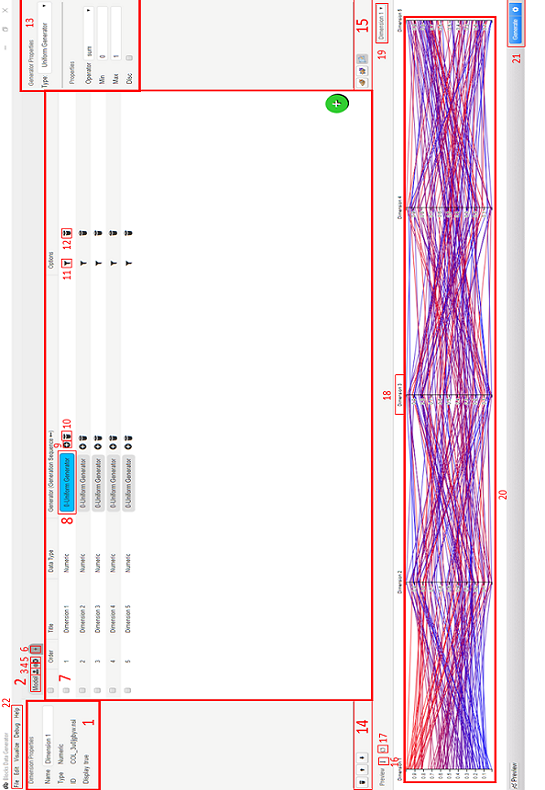
\includegraphics[width=\linewidth]{./figures/prototipo/telaprincipalmarcada.png}
			\caption{Conhecendo os elementos da tela principal do Blocks Data Generator, na sua versão para Windows. Fonte: O Autor.}
			\label{fig:telaPrincipal}
		\end{figure}
		\begin{figure}[h]
			\centering
			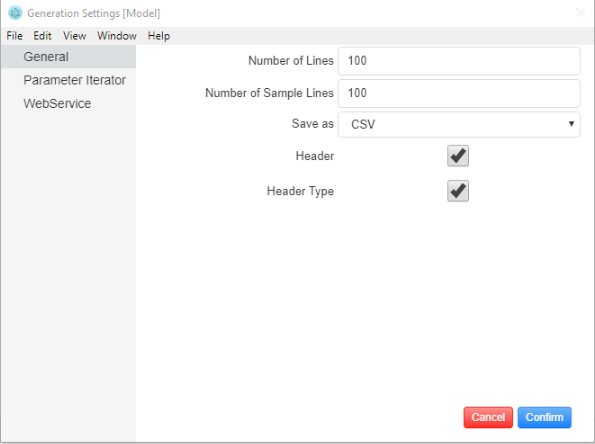
\includegraphics[width=\linewidth]{./figures/prototipo/generationSettings.png}
			\caption{Conhecendo os elementos da tela de configurações para geração de dados. Fonte: O Autor.}
			\label{fig:generationSettings}
		\end{figure}
		\par
		Na figura \ref{fig:telaPrincipal}, pode-se encontrar os principais elementos para utilizar o Blocks Data Generator.
		Na marcação 1 (M1), são definidas as propriedades da dimensão, é possível visualizar informações e alterar o título.
		A M2 mostra o nome atual do modelo, ao seu lado há o símbolo de que este modelo está servindo dados (\emph{Web Service}) (M3);
			M4 mostra que há alterações não salvas no modelo, a M5 é um botão para fechar o modelo e a M6 é para criar um novo modelo.
		\par
		A marcação 7 agrupa as dimensões do modelo. 
		A M8 é um exemplo de gerador, no formato de chip; 
			a M9 é o botão responsável por criar e aumentar o encadeamento de geradores; e a M10 excluir um gerador da cadeia - é válido ressaltar que são se pode ter menos que um gerador.
		A M11 cuida do filtro de dimensões - quando este ícone estiver com uma reta na diagonal sobre o filtro, significa que a dimensão não será incluída na geração e nem visualização dos dados.
		A M12 é um dos botões responsáveis pela exclusão da dimensão do modelo, o outro botão é encontrado na M14, junto com os botões para reorganização de dimensões - significa poder mover uma dimensão para cima ou para baixo.
		\par
		A M13 agrupa as configurações atuais do gerador. 
		Tanto as configurações da M13 quanto da M1 seguem um padrão chamado \emph{Two-way data binding}, o que signfica que não há a necessidade de um botão de salvar os dados, toda alteração é salva automaticamente, prevalecendo a consistência em todo o sistema.
		Na M13 encontra-se o tipo de gerador, que apresenta uma lista de categorias que, por sua vez, cada uma apresenta uma lista de geradores (ver seção 4.1) e também as propriedades do gerador selecionado.
		A M15 possui alguns botões que tornam a modelagem mais prática como um copiador de gerador, e (saber o que é magic painter!). 
		\par
		Na parte inferior da tela, é encontrado o pré-visualizador de dados.
		É utilizado o Coordenadas Paralelas (M20) (ver seção 4.3.1) como principal e único gráfico.
		A parte interativa deste gráfico se dá pelo \emph{ComboBox} (M19) ou pelo clique no título (ver seção 4.3.1).
		Ainda sobre o \emph{preview}, é possível escondê-lo (M16) e recarregá-lo (M17).
		Na marcação 21 encontra-se o botão para gerar os dados a partir do modelo atual e para manipular as algumas configurações o modelo atual.
		\par
		Ao clicar com o botão direito do \emph{mouse} no título do modelo (M2) aparece um menu, como visto na figura fig:contextMenu.
		Esse \emph{context menu} permite renomear ou deletar o modelo, exportá-lo como arquivo .DOT e também manipular algumas informações para o Web Service Como
			copiar para a área de transferência o ID do modelo, uma URI padrão (\emph{localhost}); ativar ou desativar o modelo pra \emph{Web Service}, bem como abrir a URI em um software padrão do usuário.
		\begin{figure}[h]
			\centering
			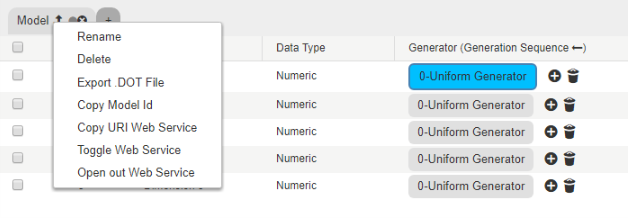
\includegraphics[width=\linewidth]{./figures/prototipo/contextMenu.png}
			\caption{Conhecendo os elementos da \emph{context menu} na aba do modelo. Fonte: O Autor.}
			\label{fig:contextMenu}
		\end{figure}
		\par
		Ao lado do botão (\emph{Generate}) para iniciar a geração é encontrado outro botão com o ícone de engrenagem (M21).
		Na imagem \ref{fig:generationSettings}, no lado esquerdo, encontra-se 3 seções.
		A primeira é dedicada para configurações gerais do modelo, como quantidade de dados para ser gerados, mostrado no \emph{preview} ou formato dos dados.
		A segunda seção (\emph{Parameter Iterator}) foi pensada para quer precisar criar mais de um arquivo variando apenas alguns parâmetros, de forma iterativa.
		A terceira seção é especial para o \emph{Web Service} no qual, liga ou desliga o servidor ou troca a porta padrão para servir os dados.
		
		\subsection{Mensagens para o usuário}
			O sistema precisa avisar o usuário de falhas, perguntar sobre preferências e afins.
			Para isso, o Blocks utiliza-se de \emph{Dialogs} (ver figura \ref{fig:dialog}) para receber um caminho para salvar ou abrir um arquivo.
			Há um espaço dedicado na tela principal para mensagens advindas de um subprocesso que está gerando dados via Streaming Data.
			Mensagem para preparação, progresso, finalização ou falha pode ser acompanhado por lá (ver figura \ref{fig:SDvisor}).
			Para outros avisos mais genéricos como erros ou tarefas bem sucedidas há o \emph{Modal} (ver figura \ref{fig:modal}).
			\begin{figure}[h]
				\centering
				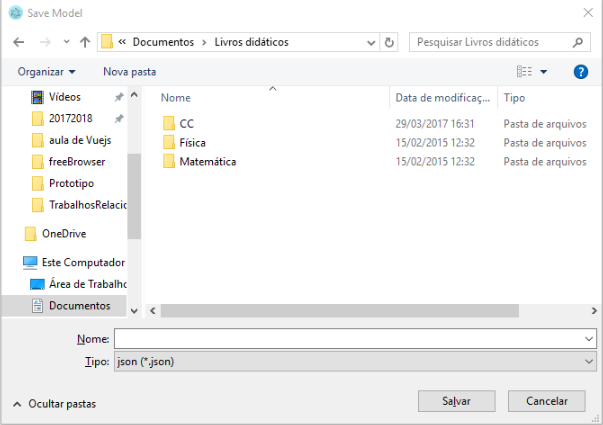
\includegraphics[width=\linewidth]{./figures/prototipo/dialog.png}
				\caption{Conhecendo os elementos da tela de configurações para geração de dados. Fonte: O Autor.}
				\label{fig:dialog}
			\end{figure}
			\begin{figure}[h]
				\centering
				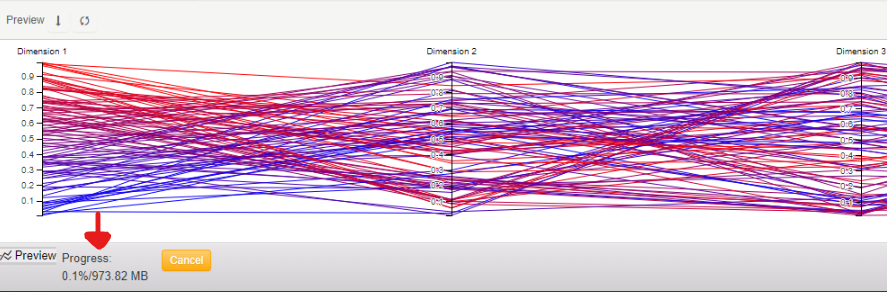
\includegraphics[width=\linewidth]{./figures/prototipo/SDvisor.png}
				\caption{Conhecendo os elementos da tela de configurações para geração de dados. Fonte: O Autor.}
				\label{fig:SDvisor}
			\end{figure}
			\begin{figure}[h]
				\centering
				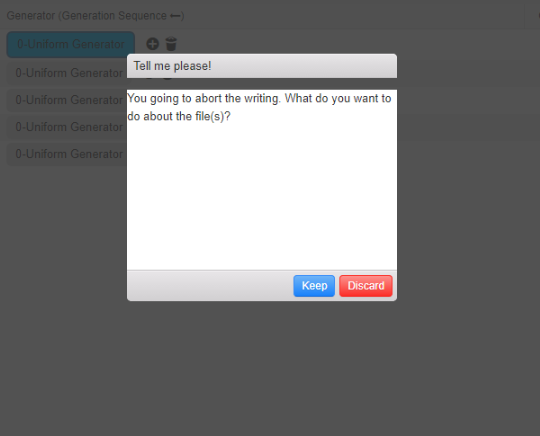
\includegraphics[width=\linewidth]{./figures/prototipo/modal.png}
				\caption{Conhecendo os elementos da tela de configurações para geração de dados. Fonte: O Autor.}
				\label{fig:modal}
			\end{figure}
		\subsection{Atalhos do Teclado}
			Modelar um conjunto de dados pode ser exaustivo, portanto, alguns atalhos podem facilitar na prevenção e correção de erros, eficiência e economia de esforço e afins.
			Visando dar praticidade ao usuário, o Block Data Generator possui atalhos para 
				criar novo modelo (Ctrl/Cmd + M);
				deletar modelo atual (Ctrl/Cmd + W);
				criar nova dimensão (Ctrl/Cmd + D);
				salvar modelo (Ctrl/Cmd + S).
			\par
			E para termos de segurança no uso, há o desfazer/refazer com Ctrl/Cmd + Z e Ctrl/Cmd + Shift + Z respectivamente.
			Além de acesso pelo teclado, os atalhos podem ser acessados pela barra superior da tela inicial (M22).
			É válido ressaltar, ainda na questão de segurança de uso, que o Blocks Data Generator salva as mudanças no automaticamente em arquivo separado, o qual pode ser recuperado se não forem salvas/descartadas adequadamente. 

			% Se sobrar tempo, fazer uns vídeos no YouTube.
			% \subsection{Ajuda}

% ---
\chapter{Resultados}
% ---
	%TODO : Não sei ainda quais são os resultados.
% Conclusão
% ---
\chapter{Conclusão}
% ---

\lipsum[31-33]

% ----------------------------------------------------------
% ELEMENTOS PÓS-TEXTUAIS
% ----------------------------------------------------------
\postextual
% ----------------------------------------------------------

% ----------------------------------------------------------
% Referências bibliográficas
% ----------------------------------------------------------
\bibliography{abntex2-modelo-references}

\end{document}
